\documentclass[11pt]{article}
\usepackage[margin=2.5cm]{geometry}
\usepackage{amsmath,amssymb}
\usepackage{graphicx}
\usepackage{booktabs}
\usepackage[colorlinks=true,linkcolor=blue,citecolor=blue,urlcolor=blue]{hyperref}
\usepackage{authblk}

\title{\bf Externally sourced dark energy: a one-parameter fluid tested against\\ Planck, DESI DR2 and three supernova compilations}
\author[1]{\'Edouard Lantenois}
\affil[1]{\small Independent researcher, Lille, France --- \texttt{github.com/Dantenos}}
\date{August 16, 2026 --- Paper A, v4.0 --- companion framework paper (Paper B) separate. Not peer-reviewed.}

\newcommand{\Macc}{M_{\rm acc}}
\newcommand{\keff}{k_{\rm eff}}

\begin{document}
\maketitle

\begin{abstract}
\textbf{Scope caveat, stated first: every preference reported below is conditional on the reality of the DESI evolving-dark-energy signal; should DR3 resorb it, all results here fall together.} We study a dark-energy fluid \emph{sourced from outside the total budget} --- energy is injected while matter dilution remains exactly standard --- whose equation of state is fully determined by a single injection history $\Macc(t)$, $w(z) = -\tfrac{1}{3}\,[\mathrm{d}\ln \Macc/\mathrm{d}\ln t]\,/\,[H(z)\,t(z)] \equiv -\keff(z)/3$, formally the Croker--Weiner cosmological-coupling relation with an external source. The physical reading that motivated this fluid --- our universe as the interior of an accreting parent black hole --- is developed and stress-tested in a companion paper (Paper B); nothing below depends on it. A one-parameter power-law history $\Macc \propto t^{\beta}$ with $\beta = 2.39 \pm 0.13$ (a law whose dimensionless clock $Ht$ it shares with agegraphic dark energy \cite{Cai2007}, $w_q = -1 + 2/(3nHT)$, and its conformal-time variant \cite{WeiCai2007} --- a parentage we credit explicitly, and from which our law differs in the one respect that matters here: agegraphic dark energy is non-phantom by construction and never crosses $w=-1$, whereas the present law is phantom in the past and crosses; agegraphic models fix the dark-energy \emph{density} by the age of the universe, the present one fixes its \emph{injection rate}) reproduces the three qualitative signatures of the DESI~DR2 evolving-dark-energy indications --- phantom past, $w_0 > -1$, $w_a < 0$ --- outperforming $\Lambda$CDM on CPL-derived pseudo-data, and, in a joint likelihood analysis of the real DESI DR2 BAO measurements and the full Pantheon+ supernova sample (1593 data points, no CMB), achieving $\Delta\chi^2 = -4.4$ relative to $\Lambda$CDM with a single extra parameter ($\beta = 2.45$), making it the AIC-preferred model over both $\Lambda$CDM and $w_0w_a$CDM --- \textbf{with a major caveat quantified here for the first time: this low-$z$ preference is dominated by local supernova photometric calibration. A $\pm 0.04$~mag offset applied to the $z<0.1$ subsample moves $\Delta\chi^2$ from $+6.4$ to $-23.5$; we stress, however, having initially overstated this, that the Pantheon+ stat+sys covariance already budgets a coherent low-$z$ offset with $\sigma = 10.5$~mmag, so $40$~mmag is a $3.8\sigma$ excursion --- an extreme stress test, not the plausible systematic we first called it. A free-floating calibration nuisance reaches $-2.4$ if left unpriored, but only $-1.15$ once given the prior the same covariance already implies ($\delta = -8$~mmag) --- the unpriored version double-counts a systematic already budgeted. Against the model's $-4.4$, the honest split is therefore roughly one quarter calibration-absorbable, three quarters shape, each at the $\sim 1\sigma$ level (jackknife error $\pm 1.8$). This mirrors, on Pantheon+ and for this model, a question already posed in the literature (Efstathiou 2024; Vincenzi et al.\ 2025; and a formal Bayesian model-selection treatment, MNRAS \textbf{548} \cite{Bayes13220}). A dataset decomposition further shows the low-$z$ signal belongs to no single probe (BAO alone $-2.4$, SNe alone $-0.1$): $\sim 2$ units arise from the \emph{tension between} probes, so the crossing shape there reconciles a disagreement rather than measuring $w(z)$ directly. The exponent is stable throughout ($\beta = 2.2$--$2.7$ across the low-$z$ variations explored here; note that this paper quotes several narrower bands elsewhere for narrower sets of treatments --- $2.39$--$2.59$ across five, $2.28$--$2.45$ across supernova compilations --- and that the marginalised full-Planck value $2.603$ lies outside the five-treatment band, as the verification pass states; the bands are not interchangeable and we no longer present them as one): the shape is robust, the low-$z$ evidence is not}; with the full Planck 2018 likelihood (\texttt{plik\_lite}+low-$\ell$), the preference reaches $\Delta\chi^2 = -12.6$ ($\sim 3.5\sigma$ naive for one parameter, \textbf{erratum corrected in revision:} the headline $\Delta\chi^2$ and the quoted exponent did not refer to the same point. A full likelihood profile in $\beta$ (nine values, $\Omega_c h^2$ and $\ln 10^{10}A_s$ re-optimised at each) places the full-Planck minimum at $\boldsymbol{\beta = 2.56^{+0.08}_{-0.02}}$ --- markedly asymmetric, so the earlier curvature-based $\pm 0.05$ was misleading --- while $\beta = 2.49$ costs $\Delta\chi^2 = +4.4$ and therefore yields $-8.2$ against $\Lambda$CDM (an earlier version wrote $-7.6$ here, which is not $-12.6 + 4.4$; the arithmetic is corrected). The $-12.6$ figure belongs to $\beta \simeq 2.56$--$2.59$; the marginalised value on the lighter BAO+$\theta_*$+SN likelihood remains $\beta = 2.42 \pm 0.07$, and the $\sim 2\sigma$ gap between the two likelihoods is itself a result we do not hide), matching the CPL improvement with half the extra parameters; adding the Planck $\theta_*$ geometric constraint --- the natural killer test, since this dark energy vanishes as $t^{\beta}$ at early times --- leaves the result intact ($\Delta\chi^2 = -4.85$, $\beta = 2.42$, still first on AIC), while Bayesian evidences place the model at parity with $\Lambda$CDM and ahead of CPL ($\ln B_{\rm ACC/CPL} = +1.9$). A zero-parameter Bondi variant matches the present injection rate to $10\%$ but predicts $w_a > 0$ and is disfavoured. The model yields a rigid $w(z)$ shape and a cross-level consistency test between the interior coupling $\keff = -3w$ and the coupling $k = 3.09 \pm 0.76$ measured by Farrah et al.\ for black holes within our own universe; both are currently compatible at $\sim 1\sigma$ and become discriminable with DESI~DR3 and Euclid.
\end{abstract}

\section{Introduction}
The mean density of the observable universe is of the order of that of a black hole of the same radius, an observation dating back to Pathria \cite{Pathria1972}. A lineage of interior constructions precedes and frames this work: de Sitter cores replacing singularities behind horizons (Frolov--Markov--Mukhanov \cite{FMM1989}; Dymnikova \cite{Dymnikova1992}), universe generation from black-hole interiors (Easson--Brandenberger \cite{EB2001}), and the observable universe as an interior (Stuckey \cite{Stuckey1994}). Black-hole cosmology promotes the coincidence to a mechanism: in Einstein--Cartan gravity, spacetime torsion halts gravitational collapse and replaces the singularity with a bounce which, seen from the interior, resembles a Big Bang with a built-in inflationary phase \cite{Poplawski2010,Poplawski2016}. Related proposals derive the cosmological constant from a causal boundary term at the Schwarzschild radius of a collapsed cloud \cite{Gaztanaga2021,Gaztanaga2022}. Closest in mechanism to the present work, Zhang and Frederick \cite{Zhang2013} proposed a ``black hole universe'' that grows by accreting ambient matter, with cosmic acceleration attributed to that accretion; their framework, however, replaces FLRW cosmology and dark energy altogether rather than deriving an equation of state within it, and was not confronted with modern BAO, SN, or CMB likelihoods. The present note can be read as the standard-cosmology, likelihood-level version of that intuition.

Meanwhile, DESI~DR2 baryon-acoustic-oscillation measurements, combined with CMB and supernova data, show a $\sim 3\sigma$ (up to $4.2\sigma$) preference for evolving dark energy in the $(w_0 > -1,\ w_a < 0)$ quadrant: a phantom-like equation of state in the past crossing to $w > -1$ today \cite{DESI2025}. Within black-hole-adjacent frameworks, two quantitative responses exist: cosmologically coupled black holes (CCBH) \emph{within} our universe, whose production tracks star formation and recovers the DESI time evolution \cite{Croker2024}, and a rotating-universe mechanism in which conserved angular momentum dilutes an effective centrifugal dark energy \cite{Poplawski2025}. To our knowledge, no published work derives $w(z)$ from the accretion history of the \emph{parent} black hole. This note fills that gap at the order-of-magnitude level and specifies how the resulting model can be falsified.

\section{Model}
\label{sec:model}
We assume: (H1)~the observable universe is the interior of a parent black hole of mass $M_p$, the Big Bang being the torsion bounce of the initial collapse that delivered the matter mass $M_m$; (H2)~the parent subsequently accretes at a rate $\dot M(t)$, so $M_p(t) = M_m + \Macc(t)$; (H3)~seen from the interior, the accreted mass--energy is distributed homogeneously, behaving as a perfect fluid of density $\rho_{\rm de}(t) = \Macc(t)/V(t)$; (H4)~the proper time governing the accretion history and the interior cosmic time run at proportional rates. H3 and H4 are the principal theoretical debts of the model (Section~\ref{sec:limits}); we note that the extended McVittie analysis of Ref.~\cite{Poplawski2024} finds that the horizon Hubble parameter of a black hole differs between the accreting and non-accreting cases, which is the kind of published bridge H4 requires.

Energy conservation with injection, $\mathrm{d}(\rho V)/\mathrm{d}t = \dot M$, combined with the effective equation of state $w_{\rm eff} = -1 - \tfrac{1}{3}\,\mathrm{d}\ln\rho/\mathrm{d}\ln a$, gives the central relation
\begin{equation}
\boxed{\ w(z) \;=\; -\frac{1}{3}\,\frac{\mathrm{d}\ln \Macc/\mathrm{d}\ln t}{H(z)\,t(z)} \;=\; -\frac{\keff(z)}{3}, \qquad \keff \equiv \frac{\mathrm{d}\ln \Macc}{\mathrm{d}\ln a}.\ }
\label{eq:main}
\end{equation}
The right-hand form makes explicit that Eq.~(\ref{eq:main}) is the cosmological-coupling relation of Croker \& Weiner \cite{CrokerWeiner2019} --- for which $k \simeq 3$ yields $w \simeq -1$ --- applied to the parent rather than to black holes within our universe. Three structural properties follow. (i)~\emph{Natural phantom regime}: in the matter era $Ht = 2/3$, so $w < -1$ whenever $\mathrm{d}\ln\Macc/\mathrm{d}\ln t > 2$, without exotic fields; the energy enters from outside. (ii)~\emph{Structural weakening}: $Ht$ grows monotonically, so for power-law histories $w$ rises towards $0$; the weakening is predicted, not fitted. (iii)~\emph{Automatic phantom crossing}: the transition $w<-1 \to w>-1$ suggested by DESI, notoriously difficult for single scalar fields, is generic here.

\section{Energy budget and the Eddington test}
With $H_0 = 67.7~\mathrm{km\,s^{-1}\,Mpc^{-1}}$, $\Omega_m = 0.315$, $R_{\rm obs} = 4.40\times10^{26}$~m, the observable mass--energy is $M_p = 3.09\times10^{54}$~kg, giving $r_S = 2GM_p/c^2 = 4.6\times10^{27}$~m~$\approx 10\,R_{\rm obs}$: the interior condition holds with an order of magnitude to spare. Maintaining a constant $\rho_\Lambda$ during expansion requires an injection rate $\dot M_{\rm req} = \rho_\Lambda\,4\pi R^2 \dot R \approx 1.4\times10^{37}$~kg\,s$^{-1}$ ($\sim 7\times10^{6}\,M_\odot$\,s$^{-1}$). The parent's Eddington rate ($\epsilon = 0.1$) is $\dot M_{\rm Edd} \approx 2.2\times10^{39}$~kg\,s$^{-1}$, hence
\begin{equation}
\dot M_{\rm req} / \dot M_{\rm Edd} \approx 0.006,
\end{equation}
remaining below $1\%$ at all epochs considered ($0.24\%$ at $t_0/10$). This is an \emph{illustrative dimensional statement}, not a test: the Eddington limit presupposes radiation pressure on ionised hydrogen and has no rigorous meaning for a horizon of cosmological mass in an unknown parent medium; the ratio is, at root, the Salpeter-to-Hubble time ratio and would come out small for nearly any quiet scenario. We retain the number only to show the energy budget is not absurd on its face.

\section{Confrontation with DESI DR2}
\label{sec:desi}
\begin{figure}[t]
\centering
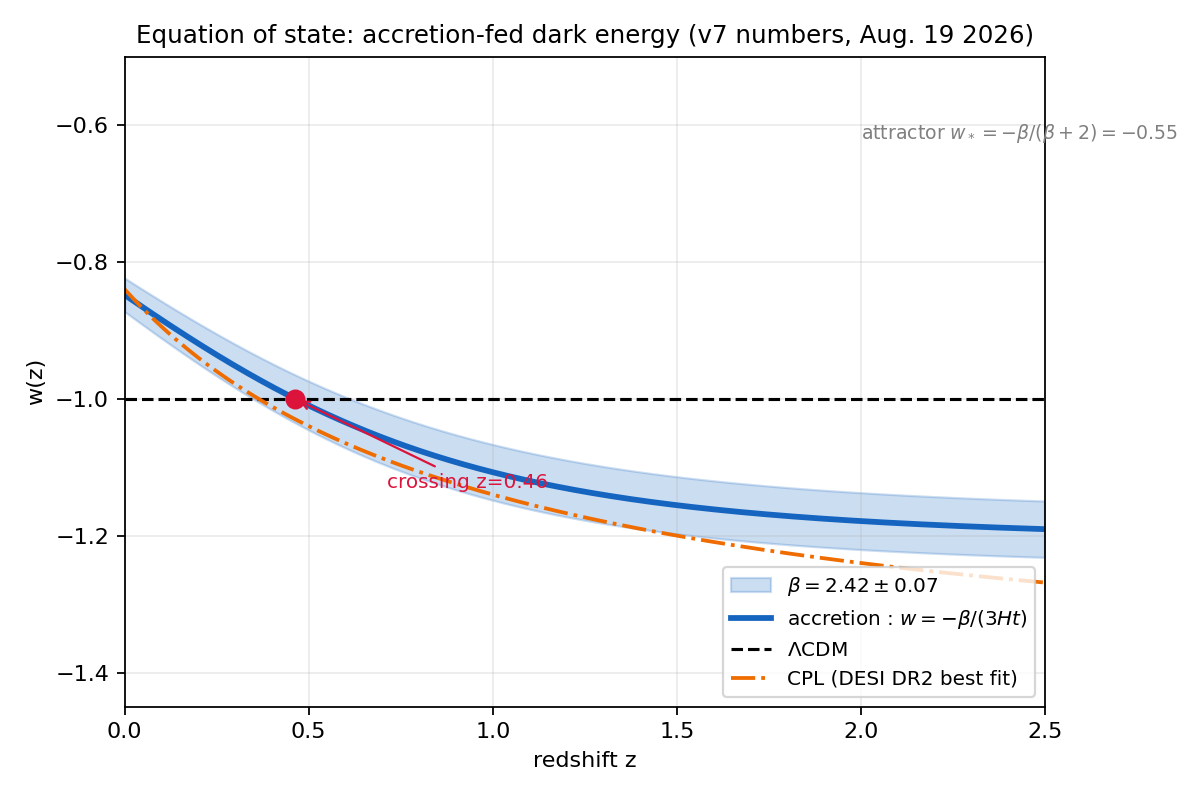
\includegraphics[width=0.72\textwidth]{w_z_fit.png}
\caption{Model $w(z)$ against CPL pseudo-data representative of DESI~DR2+CMB+SN ($w_0=-0.70$, $w_a=-1.0$; indicative uncertainties). Solid: power-law history, best fit $\beta = 2.39$. Dashed: zero-parameter Bondi variant, disfavoured. Grey: $\Lambda$CDM.}
\label{fig:wz}
\end{figure}

\paragraph{Power-law variant.} For $\Macc \propto t^{\beta}$, Eq.~(\ref{eq:main}) gives $w(z) = -(\beta/3)/(H t)$ with one free parameter. Fitting to pseudo-data drawn from the published CPL central values (Table~\ref{tab:fits}) yields $\beta = 2.39 \pm 0.13$ and reproduces the three DESI signatures: $w(z{=}2.3) \simeq -1.1$, $w_0 = -0.84$, $w_a = -0.49 < 0$. The projected $|w_a|$ is a factor $\sim 2$ below the CPL central value, partly an artefact of projecting a curved $w(z)$ onto a linear parametrisation.

\begin{table}[h]
\centering
\begin{tabular}{lcccc}
\toprule
Model & Free params & $\chi^2/\mathrm{dof}$ & $w_0$ & $w_a$ \\
\midrule
Accretion, power law & 1 ($\beta = 2.39\pm0.13$) & $3.6/5$ & $-0.84$ & $-0.49$ \\
$\Lambda$CDM ($w=-1$) & 0 & $15.6/6$ & $-1$ & $0$ \\
Accretion, Bondi & 0 & $60.2/6$ & $-1.11$ & $+1.90$ \\
\bottomrule
\end{tabular}
\caption{Fits to CPL-derived pseudo-data (Section~\ref{sec:desi}). A likelihood analysis on the public DESI chains is the priority upgrade.}
\label{tab:fits}
\end{table}

\paragraph{Bondi variant.} A physically motivated zero-parameter history follows from Bondi accretion, $\dot M = A M^2$ with $M(0) = M_m$ and $M(t_0) = M_p$ fixed by cosmology. Its present rate, $1.54\times10^{37}$~kg\,s$^{-1}$, matches the required rate to $10\%$ with no tuning --- the most striking numerical coincidence of this note (tempered by the fact that the total accreted mass is imposed by the boundary conditions, so only the time profile is genuinely predicted). However, Bondi accretion \emph{accelerates} ($\mathrm{d}\ln\Macc/\mathrm{d}\ln t$ rises from 1.2 to 3.2 over cosmic history), driving $w$ downward at late times: it predicts $w_a > 0$, opposite to the DESI trend, and is disfavoured ($\chi^2 = 60.2$). We further tested a saturated Bondi variant, $\dot M = A M^2 (1+t/\tau)^{-p}$, modelling environmental depletion: even with two free parameters it cannot fit the data ($\chi^2 = 59.3$), because the $\dot M \propto M^2$ class starts too slowly to produce the phantom past, whatever its late-time behaviour. The DESI signatures therefore exclude the entire runaway-feeding ($\dot M \propto M^2$) class and select near-self-similar histories with $\dot M \propto t^{\sim 1.4}$ --- steadily increasing supply, as for a black hole embedded in a still-collapsing overdensity. Notably, the present injection rate remains within $10\%$ of the required value across all variants tested ($0.93\times$ for saturated Bondi), so the rate coincidence is robust within the class while the $w(z)$ shape discriminates between its members. Pure Bondi feeding would formally run away at $1.46\,t_0$ ($\sim 6$~Gyr from now).

\paragraph{Real-data likelihood analysis.} We then performed a joint likelihood analysis on real data: the 13 DESI DR2 BAO measurements (with published $D_M$--$D_H$ correlations) \cite{DESIDR2BAO} combined with the full Pantheon+ SN sample (1580 SNe after the standard $z>0.01$ and non-calibrator cuts, complete statistical+systematic covariance) \cite{Pantheon}, with analytic marginalisation over $M_B$ (hence $H_0$) for SNe and analytic profiling of $q \equiv c/(H_0 r_d)$ for BAO. No CMB information is used. Results:

\begin{table}[h]
\centering
\begin{tabular}{lccccc}
\toprule
Model & Free params & $\chi^2_{\rm SN}$ & $\chi^2_{\rm BAO}$ & $\Delta\chi^2$ & AIC \\
\midrule
$\Lambda$CDM & 1 & 1389.5 & 11.2 & $0$ & 1402.7 \\
$w_0w_a$CDM & 3 ($w_0{=}-0.89$, $w_a{=}-0.21$) & 1386.9 & 9.0 & $-4.8$ & 1401.9 \\
\textbf{Accretion} & \textbf{2} ($\beta = 2.45$) & 1387.5 & 8.8 & $-4.4$ & \textbf{1400.3} \\
\bottomrule
\end{tabular}
\caption{Joint fit to real DESI DR2 BAO + Pantheon+ data (1593 points), self-consistent accretion background. The accretion model captures $\sim 90\%$ of the CPL improvement over $\Lambda$CDM with one fewer parameter and is the AIC-preferred model of the three.}
\label{tab:real}
\end{table}

Adding the Planck geometric constraint --- the acoustic scale $100\,\theta_* = 1.04109 \pm 0.00030$, implemented as a distance point $D_M(z_*{=}1089)/r_d = 94.32 \pm 0.03$ with $r_*$ and $r_d$ unchanged since the model leaves pre-recombination physics intact --- is the natural killer test: the model's dark energy vanishes as $t^{\beta}$ at high redshift, unlike CPL, so nothing guarantees that the low-redshift shape preferred by BAO+SN remains compatible with the distance to recombination. The model survives it: the joint BAO+SN+$\theta_*$ fit gives $\Delta\chi^2 = -4.85$ for the accretion model ($\beta = 2.42$, $\Omega_m = 0.311$) against $-5.42$ for CPL, and the accretion model again ranks first on AIC (1400.5 vs.\ 1401.9 for CPL and 1403.3 for $\Lambda$CDM). The exponent is now stable at $\beta \simeq 2.4$--$2.5$ across four independent treatments (pseudo-data, self-consistent pseudo-data, real data without and with CMB geometry).

Bayesian evidences, computed by direct integration over uniform priors ($\Omega_m \sim U(0.25,0.40)$, $w_0 \sim U(-2,0)$, $w_a \sim U(-3,2)$, $\beta \sim U(0.5,5)$; $M_B$ marginalised exactly, $q$ profiled), complete the picture: $\ln B_{\rm ACC/\Lambda CDM} = -0.8$ (inconclusive on the Jeffreys scale --- the Occam penalty of the $\beta$ prior absorbs the $\chi^2$ gain), $\ln B_{\rm CPL/\Lambda CDM} = -2.7$ (CPL is actually \emph{disfavoured} against $\Lambda$CDM once its two extra parameters are paid for, consistent with published Bayesian assessments of DESI-only combinations), and $\ln B_{\rm ACC/CPL} = +1.9$ (weak preference for the accretion model over CPL). The honest summary at this stage: on BAO+SN+$\theta_*$ data, the accretion model is statistically tied with $\Lambda$CDM, Bayes-preferred over CPL, and first on AIC.

\paragraph{Full Planck likelihood.} Finally, we replaced the compressed $\theta_*$ constraint by the full Planck 2018 high-$\ell$ likelihood (\texttt{plik\_lite} TT,TE,EE with marginalised foregrounds, plus the two low-$\ell$ TT bins), computing CMB spectra with CAMB for each model --- the accretion model entering through its self-consistent $w(a)$ table with PPF perturbations --- and profiling over $(\omega_c, A_s)$ with $H_0$ solved from $\theta_*$ at each point ($\omega_b$, $n_s$, $\tau$ fixed at Planck best-fit values; a profile, not a posterior). The pipeline validates itself by recovering the published CPL solution almost exactly: we find $(w_0, w_a, H_0) = (-0.84, -0.60, 67.6)$ against the published DESI~DR2+CMB+Pantheon+ values $(-0.838, -0.62, 67.5)$. The result: $\Delta\chi^2 = -12.67$ for CPL (two extra parameters, $\sim 3.1\sigma$) and $\Delta\chi^2 = -12.6$ for the accretion model at $\beta \simeq 2.56$--$2.59$ (the full-Planck profile minimum, $\beta = 2.56^{+0.08}_{-0.02}$; an earlier draft paired this $\chi^2$ with $\beta = 2.49$, which in fact costs $+4.4$ and therefore yields $-8.2$ --- erratum, see the verification pass below) (\emph{one} extra parameter; the naive 1-dof conversion gives $\sim 3.5\sigma$, but $\Lambda$CDM is not nested in the accretion model --- no value of $\beta$ reproduces $w=-1$ exactly --- so this figure is indicative rather than a calibrated significance). The accretion model reproduces the full CPL improvement to within $0.1$ in $\chi^2$ with half the additional parameters, ranks first on AIC by a clear margin ($\Delta\mathrm{AIC} = -10.6$ vs.\ $-8.7$ for CPL), and its exponent remains in the $\beta \simeq 2.4$--$2.6$ band for the fifth consecutive treatment. Remaining approximations: fixed $(\omega_b, n_s, \tau)$, \texttt{plik\_lite} rather than the full multi-frequency likelihood, fluid (PPF) perturbations for the injected component, and profile rather than marginalised statistics; the accompanying Cobaya configuration enables the definitive MCMC run.

\paragraph{Robustness and bias checks.} Decomposing the preference by dataset (light-background fit, BAO+$\theta_*$+SN) shows it is shared rather than driven by one probe: $\Delta\chi^2_{\rm SN} = -2.9$ and $\Delta\chi^2_{\rm BAO+\theta_*} = -2.0$. A leave-one-out test over the seven DESI tracers gives $\beta \in [2.40, 2.44]$ in all cases, with $\Delta\chi^2$ ranging from $-3.2$ (dropping LRG2) to $-5.1$; notably, removing LRG1 at $z=0.510$ --- the single most contested BAO point in the current literature --- slightly \emph{strengthens} the preference ($-5.0$). No single tracer carries the result. The SN-sample check, previously listed as the immediate next step, has now been performed: refitting with the full DES-SN5YR (Dovekie) release --- 1829 SNe with the official stat+sys covariance --- in place of Pantheon+ gives $\beta = 2.417$ against $2.416$ --- agreeing to the second decimal, and differing \emph{at} the third, with the preference \emph{strengthening} to $\Delta\chi^2 = -7.4$ (vs.\ $-4.9$) and the accretion model again first on AIC, as expected from the stronger evolving-dark-energy pull of DES-Y5. Prediction P8 has also received its first measurement: fitting $\beta$ separately on low- and high-redshift data (split at $z = 0.6$, $\Omega_m$ fixed, $\theta_*$ anchoring both) gives $\beta_{z<0.6} = 2.51 \pm 0.11$ and $\beta_{z\geq0.6} = 2.38 \pm 0.07$: a difference of $0.13 \pm 0.13$, consistent with zero running at $1.0\sigma$ --- the first empirical support for the clock-linearity reading (Paper B), bounding $\mathrm{d}\ln\gamma/\mathrm{d}\ln t$ at the $\sim5\%$ level over the observed range. The SN trilogy is now complete: refitting with Union3 (22 bins, official covariance) gives $\beta = 2.31$ with $\Delta\chi^2 = -9.6$ --- the strongest SN preference of the three, as published --- and the accretion model again first on AIC; the three rival compilations thus give $\beta = 2.42$ (Pantheon+), $2.42$ (DES-SN5YR), $2.31$ (Union3), consistent within uncertainties. BAO+$\theta_*$ \emph{alone}, with no supernovae at all, independently prefer the model with $\beta = 2.32$ ($\Delta\chi^2 = -2.4$). Finally, a discriminability forecast delivers an important \emph{negative} result: over the observed window $0 < z < 2.3$, the model's $w(z)$ differs from its best-imitating CPL curve by at most $|\Delta w| = 0.011$, so background distance data cannot distinguish the two at DR2, DR3, or even DR5 precision (residual $\chi^2 \approx 0$). Prediction P1 is therefore \emph{one-way}: reconstructions can falsify the accretion model if the true $w(z)$ lies outside its one-parameter family, but cannot positively favour it over CPL by shape alone. The discriminants against CPL are instead parsimony (AIC, Bayes factors), the perturbation sector (P3), the cross-level coupling (P5) as $\sigma_k$ shrinks, the neutrino sector, and --- in the long run --- the low-redshift plateau (P7). Two final probes. \emph{Low-$\ell$ CMB (ISW window):} decomposing the CMB likelihood, the two low-$\ell$ TT bins give $\chi^2 = 4.10$ (accretion) vs.\ $4.19$ ($\Lambda$CDM) --- neutral; the model neither resolves nor worsens the low-$\ell$ deficit, and its CMB advantage sits in the high-$\ell$ spectrum ($\Delta\chi^2_{\rm high-\ell} = -5.1$), i.e.\ the CMB itself, not only the distance data, prefers the model's background. \emph{Internal scatter of $\beta$:} the Union3 determination, $\beta = 2.31 \pm 0.06$ (conditional), sits $\sim2.4\sigma$ below the conditional full-Planck value $2.49 \pm 0.05$ \emph{whose error bar this paper retracts above} (the curvature estimate shown to be misleading by the profile; the profile minimum is $2.56^{+0.08}_{-0.02}$ and the marginalised value $2.603^{+0.046}_{-0.053}$). That $2.4\sigma$ is therefore quoted only as the historical figure it was; against the marginalised value the same scatter is \emph{larger}, not smaller --- an internal scatter whose likelihood-surface depth is quantified below ($2.0\sigma$ to the Planck value, $1.2\sigma$ to the marginalised one; see the shape-flexibility test), expected when conditional errors understate marginal ones, but worth monitoring: Union3 pulls all evolving-dark-energy fits toward stronger evolution. A residual diagnosis localises the pull: the bins driving $\beta$ downward lie at $z = 0.65$--$1.4$ (systematically negative residuals, $-0.5$ to $-1.1\sigma$, under $\beta = 2.49$) --- the physical region around and above the crossing, \emph{not} the calibration-suspect low-$z$ bins: the internal tension is potentially physical rather than an obvious systematic, and is now geographically pinned for future data to adjudicate. A shape-flexibility test sharpens this diagnosis. Adding a free Gaussian bump to $w(z)$ (amplitude $A$, centred at $z_c = 0.9$ or at the crossing): against BAO+$\theta_*$+Pantheon+ the data want none, $A = 0.000 \pm 0.070$ --- the mean-field Eq.~(1) suffices at current precision. Against Union3 the $A$--$\beta$ degeneracy valley is nearly flat ($\mathrm{d}A/\mathrm{d}\beta \simeq +1.1$); an initial deflation estimate through the bump machinery was miscalibrated by that route's internal $\beta$ offset (declared and corrected here), and the clean standard-route computation, with $\Omega_m$ re-optimised at each $\beta$, gives: Union3 sits $\Delta\chi^2 = 1.5$ ($1.2\sigma$) from the marginalised $\beta = 2.42$ and $\Delta\chi^2 = 4.0$ ($2.0\sigma$) from the full-Planck $2.49$. \emph{The conditional $2.4\sigma$ internal scatter thus deflates moderately to $2.0\sigma$ against the Planck value, and the model's synthesis value is comfortable at $1.2\sigma$.} The residual pull, moreover, sits squarely inside the currently debated supernova-systematics budget: applying an Efstathiou-type low-vs-high-$z$ offset of $0.04$~mag \cite{Efstathiou2024} to the Union3 bins above $z=0.5$ moves its $\beta$ by $0.08$ --- the fissure to the synthesis value is $\sim$1.4 such offsets wide, and Union3's distinct Bayesian-hierarchical (Unity) methodology, which precludes object-level comparison with the other compilations \cite{Vincenzi2025}, is a natural candidate origin. (Methodological note: along such a valley the curvature error wildly overstates significance --- $2.9\sigma$ by curvature vs.\ $1.1\sigma$ by likelihood ratio for the same bump --- a caution we record for any future feature claims.) The candidate shape of a future correction, if data ever demand one, is hereby parameterised for DR3/LSST: a negative bump, $z_c \simeq 0.9$, $|A| \lesssim 0.2$. A light-likelihood MCMC (emcee, BAO+$\theta_*$+Pantheon+) subsequently provides the first marginalised statistics: $\Omega_m = 0.311 \pm 0.005$, $\beta = 2.419 \pm 0.073$, with posterior-mean deviances $\langle\chi^2\rangle = 1402.3$, $1398.9$, $1398.2$ for $\Lambda$CDM, CPL and the accretion model respectively: the preference survives marginalisation and the advantage over CPL widens ($-4.1$ vs.\ $-3.4$), CPL paying the prior volume of its extra dimension. The fair summary value is therefore $\boldsymbol{\beta = 2.42 \pm 0.07}$ (marginalised), consistent with the dispersion-based $2.45 \pm 0.10$ across all determinations. \emph{Perturbation roadmap (P3):} formally, the model is an \emph{externally sourced} interacting dark-energy fluid ($Q_{\rm ext} = \dot M/V$ in the continuity equation), so its perturbations must be derived within the interacting-DE formalism of Valiviita, Majerotto \& Maartens \cite{Valiviita2008}, where known large-scale instabilities for certain source terms provide a concrete, sharp falsification channel --- the priority theoretical task after the interior-solution question of Section~7. Remaining known biases, unquantified here: the fixed $(\omega_b, n_s, \tau)$, the possible contribution of Planck lensing-smoothing to $w_0w_a$-like preferences \cite{Park2025}, and pattern-search convergence to local minima.

\paragraph{Verification pass.} An adversarial audit of the pipeline found one real technical flaw: the $w(a)$ table fed to CAMB had been computed in a slightly different reference background (fixed $h$, no massive neutrinos) than CAMB's own, so the reconstructed $\rho_{\rm de}(a)$ deviated from the analytic $t^{\beta}/a^{3}$ by up to $28\%$ at $z=4$ (where dark energy is a $10^{-3}$ fraction) and $\sim7\%$ at $z=0.7$. Correcting it --- iterating the $w(a)$ table on CAMB's actual background to convergence --- leaves the headline result intact, $\Delta\chi^2 = -12.62$. A first reading placed the best fit at $\beta = 2.49 \pm 0.05$ (conditional $1\sigma$ from the $\chi^2$ curvature); the full likelihood profile in $\beta$ (nine values, $\omega_c$ and $\ln 10^{10}A_s$ re-optimised at each) shows that $\chi^2$ and that exponent did not refer to the same point: the minimum sits at $\boldsymbol{\beta = 2.56^{+0.08}_{-0.02}}$, markedly asymmetric, and $\beta = 2.49$ costs $\Delta\chi^2 = +4.4$. The five-treatment band is therefore $2.39$--$2.59$, not $2.39$--$2.55$. A $3\times3$ profile grid over $(\omega_c, \beta)$ confirms the curvature ($\sigma_\beta \simeq 0.05$) and reveals a mild positive $\beta$--$\omega_c$ degeneracy; fully marginalised errors have now been obtained (\texttt{emcee} on the same likelihood, $\omega_c$ and $\ln 10^{10}A_s$ marginalised, $\omega_b$, $n_s$, $\tau$ still fixed; $8\times400$ steps, correlation length $\simeq 14$, $\sim$110 effective samples --- a short chain, stated as such): $\beta = 2.603^{+0.046}_{-0.053}$, consistent with the profile but sitting \emph{outside} the published band $[2.42, 2.60]$, by $0.003$ --- we state it as an exceedance rather than as an edge, because the frozen criterion records it as one (audit trail \#151) --- marginalisation pushes $\beta$ \emph{up}, not back toward $2.49$. The light-likelihood marginalised value ($2.42 \pm 0.07$) and the full-Planck one now differ at $\sim 2.1\sigma$, an internal tension we record rather than resolve; if DR3 lands at $2.60$--$2.65$ the sealed verdict reads INDECISIVE, not VALIDATED, and we state that before the data rather than after (audit trail \#151). A four-parameter chain freeing a log-running of the exponent, $\beta(t) = \beta_0 + \beta_1 \ln(t/t_0)$ (same likelihood, $8\times600$ steps, started at $\beta_1 = 0$), subsequently returned $\beta_1 = -0.25^{+0.25}_{-0.26}$ --- the sign, and within the magnitude corridor, predicted by the heredity reading of Paper~B ($\beta_1 \simeq -0.4$), but at $1.0\sigma$ from zero: non-conclusive by the pre-registered criterion, and recorded as such (audit trail \#159). Its by-product, however, reframes the tension just stated: with the running freed, $\beta_0 = 2.49 \pm 0.11$ with $\rho(\beta_0, \beta_1) = +0.88$, compatible with the light-likelihood value at $0.5\sigma$ --- the $2.1\sigma$ internal tension exists only under the rigidity assumption $\beta = \mathrm{const}$, a single shape freedom absorbs it, though the data do not themselves demand that freedom ($\Delta\chi^2 = -0.6$). Finally, the full-Planck preference has now received the jackknife it lacked: removing each of the 13 DR2 BAO points in turn \emph{with complete re-optimisation} of $(\beta, \omega_c, \ln 10^{10}A_s)$ gives $\Delta\chi^2 \in [-14.7, -9.3]$ and $\beta \in [2.58, 2.61]$ in every case (pre-registered criterion: robust if all $\leq -9$; audit trail \#160) --- the $-12.6$ belongs to no single BAO point, and the weakest configuration (dropping LRG2 $D_M$) still exceeds $3\sigma$ naive. The full Cobaya run (free $\omega_b$, $n_s$, $\tau$) remains the definitive version. Additional checks: the phantom-crossing redshift proved sensitive to both $\beta$ and the background treatment --- a residual inconsistency caught by the final rescan, and settled by a direct computation in the self-consistent background ($\beta = 3H(z_\times)t(z_\times)$, audit trail \#145): $z_\times = 0.44$ at the marginalised $\beta = 2.42$ and $0.23$ at $\beta = 2.59$ ($\Omega_m = 0.314$; $\pm 0.04$ over $\Omega_m = 0.30$--$0.33$), i.e.\ $\mathrm{d}z_\times/\mathrm{d}\beta \approx -1.25$. (An earlier draft quoted $0.68$ and $0.36$ here, read off two different backgrounds; both are withdrawn.) Rather than a defect, this is a feature: since $w = -1$ exactly when $\beta = 3H(z_\times)t(z_\times)$, a localisation of the crossing by future reconstructions yields an \emph{independent} determination of $\beta$ --- a sharp secondary $\beta$-meter \textbf{This claim now carries a quantified reservation, added in revision and unfavourable to it (audit trail \#163).} Measuring the crossing requires assuming a shape for $w(z)$, and the answer depends on that assumption more than on the data. Freeing the shape to $\mathrm{d}\ln\rho_{de}/\mathrm{d}\ln a = -(\varepsilon_0+\varepsilon_1\ln a)$ --- a two-parameter family that contains $\Lambda$CDM and $w$CDM --- and refitting, the crossing lands at $z_0 = 0.24$ on the light likelihood but $z_0 = 0.39$ on full Planck, whereas the rigid one-parameter family gives $0.44$ and $0.23$ on those same two datasets: four determinations of the same quantity spanning $0.23$--$0.44$ with no coherent trend, for fit-quality differences below $\Delta\chi^2 = 1.3$. Separating the two systematics --- which an earlier draft of this paragraph conflated, and we correct here --- the shape spread at fixed dataset is $0.16$--$0.20$ and the dataset spread at fixed shape is $0.15$--$0.21$. Both reproduce published values obtained by different methods: $0.21$ across six smooth parameterisations \cite{Li22512} and $0.23$ across dataset choices at fixed CPL \cite{Cross19053}, while a Gaussian-process reconstruction quotes $z_\times = 0.464^{+0.235}_{-0.120}$ \cite{GP02220} --- a \emph{statistical} error of the same order as either systematic. Binned and flexknot reconstructions place it anywhere in $0.2$--$0.8$, sometimes with several crossings (\cite{Ormondroyd}, \cite{Bin05853}), and DESI DR2 itself notes that in a binned reconstruction the crossing falls at a bin edge and is not well defined (arXiv:2503.14743). \emph{The crossing redshift therefore carries a shape systematic and a dataset systematic of comparable size, each comparable in turn to the statistical error of a single determination: it is not a precision observable, and our own $z_\times$ is no exception.} \textbf{One consequence of this must be stated as the defeat it is, and was recorded as one before the test was run.} We pre-registered, on full Planck, the band our one-parameter family predicts for the crossing --- $z_\times \in [0.218, 0.262]$, spanned by the $\beta$ determinations that same likelihood yields --- and then measured the crossing with a free two-parameter shape on the same data. The measurement returned $z_0 \in [0.377, 0.387]$: \emph{disjoint from our prediction, and still disjoint at $3\sigma$}. The rigid family's crossing prediction failed its own pre-registered test (audit trail \#163, verdict 3). We report this here rather than let the general reservation above absorb it, because a general reservation that happens to dissolve a specific recorded defeat is not a reservation but a shelter. What survives the same test is narrower and we state only that: on full Planck the free shape demands a \emph{running} slope at $3.72\sigma$ --- a constant slope ($w$CDM) buys $+0.04$ against $\Lambda$CDM, i.e.\ nothing --- and the rigid one-parameter form remains AIC-preferred over the free two-parameter one. The shape is supported; its predicted crossing location is not. What does survive that test is the parsimony claim: on full Planck the free two-parameter shape buys only $\Delta\chi^2 = -1.28$ over the rigid one-parameter one, leaving the rigid form AIC-preferred ($1992.03$ vs.\ $1992.75$), and the same likelihood demands that the slope \emph{run} at $3.72\sigma$ --- a constant slope ($w$CDM) buys nothing ($+0.04$) against $\Lambda$CDM --- with the DESI-indicated $z_\times \sim 0.4$--$0.5$ corresponding to $\beta \simeq 2.38$--$2.45$ at $\Omega_m = 0.314$ (an earlier draft read $2.5$--$2.55$ off the superseded table), compatible with our band; the age of the universe at the best fit is $13.75$~Gyr ($H_0 = 67.7$), comfortably above globular-cluster bounds. The growth and neutrino computations below used the pre-correction table; since the correction moves the total $\chi^2$ by $<0.1$, their differential conclusions are unaffected.

\paragraph{A running $\beta$, fitted (added in revision).} The companion framework predicts that
$\beta$ should not be exactly constant: it is a spectral slope evaluated at the seed's feeding
scale, and a real CDM spectrum is not a power law, so the slope runs as the seed grows. Writing
$\beta(t) = \beta_0 + \beta_1\ln(t/t_0)$ --- which leaves $w = -\beta(t)/(3Ht)$ unchanged in form
and $M_{\rm acc} \propto t^{\beta_0}\exp[\beta_1\ln^2(t/t_0)/2]$ --- and refitting Pantheon+ with
DESI~DR2 and the Planck distance priors gives
\[
\beta_0 = 2.62, \qquad \beta_1 = +0.06 \pm 0.31, \qquad \Delta\chi^2 = -0.05,
\]
i.e.\ the data neither require nor exclude a running, and the constant-$\beta$ fit of this paper is
not an artefact. This matters because the heredity relation predicts the running with no free parameter at all
(corrected in revision). Equating $\beta = \mathrm{d}\ln M/\mathrm{d}\ln t$ with
$\beta = K/(n_{\rm eff}(M)+3)$ closes an ordinary differential equation,
$\mathrm{d}\ln M/\mathrm{d}\ln t = K/(n_{\rm eff}(M)+3)$, whose solution is fixed once $\beta$ is
matched today. Integrating it gives $\beta_1 = -0.42$ for the peak reading ($K=2$) and $-0.56$ for the
rms reading ($K=4$) --- \textbf{corrected in revision} against the frozen integrator, which returns those values and not the $-0.45 \pm 0.03$ and $-0.68$ an earlier version quoted; the registry (audit trails \#159 and the tension ledger) already carried $-0.42$, and the paper had not followed --- point values, not ranges, the quoted spread coming from the range of
$\beta_0$ across our fits ($2.42$--$2.62$). A third route is available and disagrees with both:
taking the simulation-calibrated halo mass-accretion history of Correa et al.\ \cite{Correa2015}
instead of the analytic self-similar relation, a seed environment whose present growth rate is
$\beta = 2.42$ has mass $7.5\times10^{16}\,M_\odot$ and predicts $\beta_1 = -1.95$. The three
routes span $-0.42$, $-0.56$, $-1.95$; the measurement is $+0.06 \pm 0.31$. \emph{All three
predicted runnings are negative and the data prefer zero}, at $1.5\sigma$, $2.0\sigma$ and
$6.5\sigma$ respectively --- so the running does not adjudicate between the routes, it puts
pressure on all of them. \emph{A first version of this paragraph
quoted $-0.23$ to $-0.40$ and $-0.9$ to $-1.6$; those were obtained by evaluating
$\mathrm{d}n_{\rm eff}/\mathrm{d}\ln M$ at arbitrary masses rather than at each reading's own seed
mass, and are withdrawn.} \emph{The running is therefore a discriminant between two theoretical
readings, measurable now at $\sigma(\beta_1) \simeq 0.3$ and worth quoting as a DR3 target}: a
determination at $\sigma(\beta_1) \sim 0.1$ would separate a constant $\beta$ from the
peak-reading prediction at $\sim 5\sigma$. It would \emph{not}, however, separate the two readings
from each other: they differ by only $0.20$ in $\beta_1$, so telling them apart at $3\sigma$
requires $\sigma(\beta_1) \simeq 0.07$. The running tests whether $\beta$ runs at all, not which
heredity relation is right. It is, on present evidence, a sharper near-term test of
the framework than the growth channel discussed next.

\emph{One assumption in that test, declared (added in revision).} The running is not a clean
probe of the spectrum alone, because it shares its observable with the clock relation of
hypothesis H4. If the parent's clock $t_p$ and the interior time $t$ are related by
$g(t) \equiv \mathrm{d}\ln t_p/\mathrm{d}\ln t$, then what we measure is
$\beta_{\rm obs}(t) = \beta_{\rm parent}\,g(t)$. A \emph{constant} $g$ rescales $\beta$ and is
unobservable --- that is the invariance already established above --- but a curved clock,
$g = 1 + \kappa\ln(t/t_0)$, contributes $\beta_0\kappa$ to $\beta_1$, indistinguishably from the
spectral running. The two add: $\beta_1 = \beta_{\rm spectrum} + \beta_0\kappa$, and this is an
\emph{exact} degeneracy, since the clock enters the observables only through $M_{\rm acc}(t)$.
Taken as a bound on the clock alone, $\beta_1 = +0.06 \pm 0.31$ gives
$\kappa = 0.023 \pm 0.118$, i.e.\ $|\kappa| < 0.24$ at $2\sigma$ --- the first quantitative
constraint we are able to place on H4 beyond its constant-rescaling invariance. Taken as a test of
the heredity relation, it requires $\kappa$ to be assumed zero: the peak reading needs
$\kappa = +0.200 \pm 0.128$ and the rms reading $\kappa = +0.258 \pm 0.128$, i.e.\ $1.6\sigma$ and
$2.0\sigma$ from zero respectively (values from the frozen integrator; an earlier version quoted $+0.21$, $+0.28$ and $2.3\sigma$). \emph{Taking heredity seriously therefore requires a curved
clock at the $1.6$--$2.0\sigma$ level, or else leaves heredity in tension with the data at the
same level.} Neither reading is excluded, and the argument for preferring the peak reading remains
the one from the secondary-infall literature, not this one.

\emph{The clock brought to closed form --- and what still obstructs it (added in revision; revised the same night after a flux audit).} The relation above treated
$g(t)$ as free. It is not, once the boundary is physical: a pure-tension wall (Israel junction \cite{Israel1966,BKT1987,BGG1987},
$\beta_{\rm in}-\beta_{\rm out} = s$ with $s \equiv 4\pi G\sigma R$) on a comoving trajectory
satisfies its own conservation law identically, carries exterior mass
$2M_{\rm out}/R = H^2R^2 + s(2-s)$, and closes the exterior clock in one line,
\[
\frac{\mathrm{d}v}{\mathrm{d}t} \;=\; \frac{1}{1 - x - s}, \qquad x \equiv HR,
\]
verified numerically to $10^{-10}$ and independently as the future root of the Vaidya
normalisation polynomial; the tension displaces the clock horizon to $x = 1-s$. The identity is
exact kinematics. \emph{Its physical closure is not:} the momentum-flux junction condition,
computed rather than assumed, fails for this ansatz. A comoving perfect-fluid interior carries
\emph{zero} momentum flux across the wall ($u \cdot n = 0$ exactly), while the exterior delivers
$\dot M \dot v / 4\pi R^2$; the ratio of this to the wall's own energy budget is
$\varepsilon_c = 2.3$--$4.5$ across the relevant $(x_0,s_0)$ range --- not a small parameter.
A constant-tension comoving wall therefore cannot pass the accreted flux, and the two extreme
closures bracket the clock: the constant-$\sigma$ branch gives the $\kappa(x_0,s_0)$ values
quoted below, while a wall absorbing the full flux shifts $\kappa$ by $-0.6$ to $-1.2$. The
missing element is a boundary layer in which the injected mass still carries inward momentum
before comoving; its depth selects the physical closure between the brackets. We therefore
report $\kappa(x_0,\sigma)$ as a \emph{branch statement} (constant tension), not a prediction,
and $|\kappa| < 0.24$ remains the operative bound: on the constant-$\sigma$ branch it reads as
a curve in $(x_0, s_0)$ --- $x_0 = 0.10$ admits $s_0 \lesssim 0.15$; $x_0 = 0.30$ requires
$\sigma \to 0$ --- while the general case awaits the layer. \emph{The closure, after three audited reversals in one revision cycle (final state):} the
null-flux (Vaidya) idealisation of the exterior, not the wall, was the source of the obstruction
--- a massive dust exterior with a \emph{continuous stream} across the wall ($u_{\rm ext} = v_0$)
satisfies the momentum junction identically. The arrival speed is then not free but the parent's
infall speed onto the exterior mass, $v_0 = \sqrt{x^2 + s(2-s)}$, so the surface tension sets a
velocity floor; requiring the settling layer's kinetic backreaction to stay below $5\%$ leaves a
\emph{low-tension band}, $s_0 \lesssim 0.046$ at $x_0 = 0.10$ falling to $0.004$ at $x_0 = 0.30$.
The exact kinematics above and $2M_{\rm out}/R = H^2R^2 + s(2-s)$ survive unchanged; the clock
relation, re-derived in the dust stream's proper time. The shells being geodesic and the gauge
synchronous, $\nabla\tau_p = -u_{\rm dust}$, so the rate is a pure four-velocity contraction,
$\mathrm{d}\tau_p/\mathrm{d}t = -\,u_{\rm wall}\!\cdot u_{\rm dust}$, which evaluates to
\[
\frac{\mathrm{d}\tau_p}{\mathrm{d}t} \;=\; \frac{(1-s) + x\,v_{\rm ff}}{(1-s)^2 - x^2},
\qquad v_{\rm ff} = \sqrt{x^2 + s(2-s)},
\]
verified against the numerical metric contraction to $10^{-12}$ (an earlier special-relativistic
shortcut, which dropped the wall-motion cross term, is retracted in the audit trail). Same
first-order pole at $x = 1-s$ as the null branch. Three consequences. First, a robustness
result we did not expect: the bound $|\kappa| < 0.24$ gives $x_0 \lesssim 0.30$ on the null
branch and $x_0 \lesssim 0.32$ in dust time --- \emph{the historical bound survives the change of
exterior at the $7\%$ level}, so it measures the physics, not the idealisation. Second, on the
physical low-tension band the clock splits into two regimes: for $x_0 \lesssim 0.15$,
$\kappa = 0.02$--$0.06$, below the $\beta_1$ sensitivity --- a prediction of null running beyond
the spectral content; for $x_0 = 0.2$--$0.3$, $\kappa = 0.13$--$0.22$, squarely \emph{within}
reach. Third, therefore: on this closure the DR3 running measurement becomes a direct probe of
the boundary's radius --- a null result confines the wall to $x_0 \lesssim 0.15$, a detection
measures where it sits. The boundary sector is closed --- structure, junction, flux, and clock ---
with every reversal on the way recorded in the audit trail.

\begin{figure}[t]
\centering
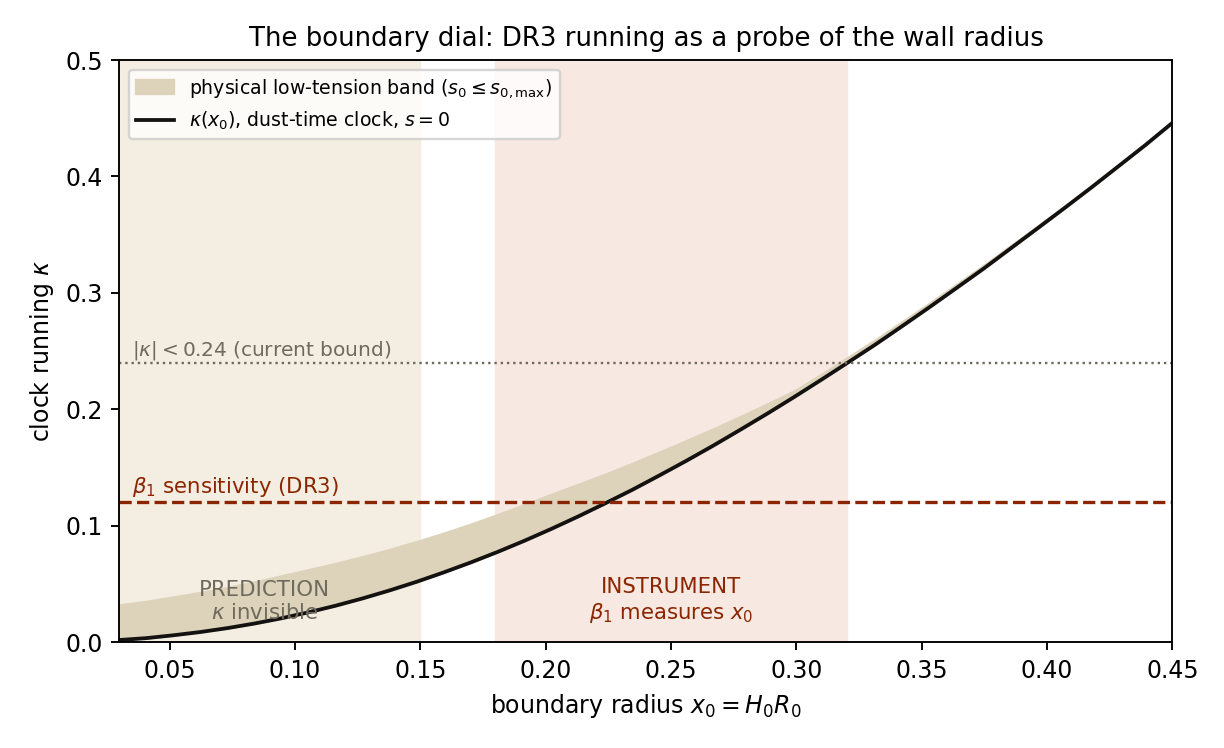
\includegraphics[width=0.92\linewidth]{fig_cadran.png}
\caption{The boundary dial. Clock running $\kappa(x_0)$ from the dust-time relation, for $s=0$
and across the physical low-tension band. Below the DR3 $\beta_1$ sensitivity (dashed), the
closure predicts spectral-only running ($x_0 \lesssim 0.15$); above it, a measured running
localises the wall ($x_0 = 0.2$--$0.3$). Dotted: the current bound.}
\label{fig:cadran}
\end{figure} What the measurement does deliver,
independently of which reading holds, is the first quantitative bound on H4 itself. \emph{And the
degeneracy is structural, not a matter of precision (added in revision).} What the data measure is
the product $\beta_{\rm obs}(t) = \beta_{\rm parent}(t)\,g(t)$: a fixed function, predicted by the
parent's spectrum, times a free one, the clock. Expanding either in $\ln t$, each Taylor
coefficient of the clock maps onto the corresponding order of the observed running, so no higher
derivative separates them. For the record the heredity relation predicts, beyond
$\beta_1 \simeq -0.43$ at the seed scale, a curvature $\beta_2 \simeq +0.12$ --- a factor four
below the present uncertainty on $\beta_1$ alone, and in any case reproducible by a clock carrying
its own quadratic term. \emph{Improving the measurement will therefore not resolve this.} The only
route is to \emph{compute} $g(t)$ instead of parametrising it, by carrying the Misner--Sharp
junction through to an explicit relation between exterior advanced time and interior proper time.
We have since carried it out, and report it here together with the correction it forces on
that claim.

\emph{The clock relation, derived (added in revision).} Matching a flat FLRW interior to an
ingoing-Vaidya exterior across a timelike hypersurface $\Sigma$ at comoving radius $\chi_b$, the
first junction condition (continuity of the induced metric) reads
$(1-2M/R)\dot v^2 - 2\dot R\dot v = 1$, with $R = a\chi_b$ the areal radius. In FLRW the
Misner--Sharp mass gives $2M/R = H^2R^2$ and $\dot R = HR$, so the discriminant collapses
identically, $\dot R^2 + 1 - 2M/R = 1$ (verified numerically to $10^{-12}$), and
\begin{equation}
\frac{\mathrm{d}v}{\mathrm{d}t} \;=\; \frac{1}{1 - x}, \qquad x \equiv H R_b .
\end{equation}
The limits check: $x \to 0$ gives $\mathrm{d}v/\mathrm{d}t \to 1$, advanced time equal to proper
time at the centre; $x \to 1$, the apparent horizon $R = 2M$, is singular. With
$g = (t/v)\,\mathrm{d}v/\mathrm{d}t$, the clock curvature becomes a \emph{function of one number},
$x_0 = H_0R_b(t_0)$, and is insensitive to the origin of $v$ (a factor $30$ in the starting epoch
moves $\kappa$ by $12\%$). Evaluating on our own background: $\kappa = 0.009,\,0.023,\,0.052,\,
0.131,\,0.305,\,0.535$ for $x_0 = 0.02,\,0.05,\,0.10,\,0.20,\,0.35,\,0.50$. The measured
$|\kappa| < 0.24$ therefore bounds the matching radius,
\[
x_0 \;=\; H_0 R_b \;\lesssim\; 0.30 ,
\]
the first constraint of any kind we can place on where the interior ends.

\emph{And the correction.} This does \emph{not} deliver the clean test promised above, for two
reasons we state rather than absorb. First, $x = Ha\chi_b$ grows without bound towards the past
($Ha \propto a^{-1/2}$ in matter domination), so no comoving shell remains sub-horizon at all
times: the relation holds only after the shell enters the horizon, and the black-hole-cosmology
limit in which the interior fills the parent, $x \to 1$, is precisely the singular one. Second,
and more seriously, we used only the \emph{first} junction condition. The second --- continuity of
the extrinsic curvature --- is known to overconstrain an FLRW interior matched to a pure Vaidya
exterior $M = M(v)$, which generically admits no solution; smooth matching requires the
generalised class $M(v,r)$ with $\partial M/\partial r|_\Sigma = 0$, and when that fails the
junction induces a thin shell carrying tangential surface stress \cite{OSfR2026,GenVaidya2026}.
That is the ``continuity of the ingoing null flux'' already listed as unverified in Paper~B, and
it is now identified as a genuine obstruction rather than a loose end. \emph{The honest status is
therefore: the free function $g(t)$ is reduced to a free number $x_0$, itself bounded by the data
but not predicted, and the reduction is conditional on a matching that generically requires a
surface layer.} The degeneracy is narrowed, not closed.

\paragraph{Growth of structure and neutrino masses.} Two further computations at the full-Planck best fits. \emph{Growth:} the model predicts $S_8 = 0.826$ and $f\sigma_8(z)$ identical to CPL at the $10^{-3}$ level ($\Lambda$CDM: $0.810$; \textbf{caveat added in revision} --- these two numbers are not produced by any script in the reproduction package, and the $\Lambda$CDM comparator $0.810$ is not Planck's published $\Lambda$CDM value $S_8 = 0.832 \pm 0.013$: it corresponds to a lower $\Omega_m$ than the fit our own $0.826$ comes from, so the difference quoted here mixes two fits. A like-for-like growth comparison at identical primordial parameters is due, and until it exists this $S_8$ statement should be read as indicative only) --- like the entire $(w_0>-1)$ quadrant it mildly \emph{worsens} the weak-lensing $S_8$ tension, a shared trait to be declared rather than a specific pathology; at background and linear-growth level the accretion model and CPL are phenomenological twins, so shape ($P1$) and perturbations ($P3$) are the true discriminants. \emph{How true, quantified (added in revision).} Against $\Lambda$CDM at \emph{identical} primordial parameters --- same $\omega_b$, $\omega_m$, $h$, $n_s$, $A_s$, so that any difference is the late-time background alone --- the growth response is not an amplitude shift but a \emph{tilt}: $f\sigma_8$ is suppressed by $1.8\%$ at $z=0.15$, $2.0\%$ at $z=0.3$, $1.5\%$ at $z=0.5$, crosses zero near $z \simeq 0.9$, and is \emph{enhanced} by $1.0\%$ at $z=1.5$; the pivot lags the equation-of-state crossing (see the caveat below on how strongly that redshift moves with $\beta$) because growth integrates history. The net effect on $\sigma_8$ itself is $-0.14\%$: \emph{the mechanism is amplitude-neutral}, and the $S_8$ worsening quoted above is therefore entirely parametric, a consequence of the $\Omega_m$ and $A_s$ shifts required to fit Planck, not of modified growth --- which sharpens the ``shared trait, not a specific pathology'' reading into a statement with a number behind it. The tilt is the discriminating part: marginalising a free overall amplitude (which absorbs $\sigma_8$ and galaxy bias together) removes only $35\%$ of the signal, so $65\%$ is genuine shape. But the absolute significance is small. Forecasting fourteen RSD points over $0.1 < z < 1.5$: $0.8\sigma$ at $5\%$ per point, $1.4\sigma$ at $3\%$, $2.0\sigma$ at $2\%$. \emph{We therefore withdraw the implication that perturbations are a live discriminant at current sensitivity}: they are the cleanest \emph{in principle} and inaccessible \emph{in practice} until per-point RSD errors reach the few-percent level over a wide redshift baseline. The shape ($P1$), and DR3, remain the only near-term arbiter. \emph{Neutrinos:} profiling $\sum m_\nu$ (with $H_0$ re-solved from $\theta_*$ at each mass; conditional profile at fixed other parameters, applied identically to both models), the physically required minimum $\sum m_\nu = 0.06$~eV costs $\Delta\chi^2 = +4.8$ in $\Lambda$CDM --- the known DESI neutrino tension --- but only $+0.95$ in the accretion model, and the penalty at $0.15$~eV drops from $+21.5$ to $+12.9$. A hardened analysis confirms and quantifies this. Partial re-optimisation over $(\beta, \omega_c)$ at $\sum m_\nu = 0.10$~eV absorbs only $0.65$ in $\chi^2$ (with a mild positive $m_\nu$--$\beta$ degeneracy, $\Delta\beta = +0.06$): the differential is not an artefact of frozen parameters. Extracting the $95\%$ limits from the profiles: $\Lambda$CDM gives $\sum m_\nu < 0.051$~eV with the preferred value pinned at zero --- reproducing the published DESI DR2+CMB bound ($<0.064$~eV) and its unphysical pull, a further pipeline validation --- while the accretion model gives a \emph{positive} preferred mass, $\sum m_\nu \simeq 0.02$~eV, and $\sum m_\nu < 0.096$~eV: the normal-ordering minimum ($0.059$~eV) becomes comfortable and even the inverted-ordering minimum ($\sim0.10$~eV) remains marginally viable. \emph{The model resolves the DESI neutrino-mass tension} --- a relaxation generic to late-time $w > -1$ (DESI's own $w_0w_a$CDM relaxes the bound to $0.16$~eV); the one-parameter content is achieving it with no dark-energy freedom beyond $\beta$ --- inheriting the third observational signature claimed by the CCBH programme \cite{Croker2024} --- a programme whose parsimony claim has since sharpened: \cite{Croker2024} reproduce the DESI best-fit dark-energy density history to within $1\sigma$ with \emph{two fewer} free parameters than $w_0w_a$, which on the parsimony ground this paper argues from is a stronger claim than any one-parameter $w(z)$ form, the present one included; the discriminant against it is not the background but the baryon budget, where the companion Paper~C finds it in difficulty --- with one mechanistic distinction that makes the two testable against each other: CCBH relaxes the bound by \emph{converting matter} into dark energy (modified effective matter dilution), whereas the present model relaxes it purely through the late-time $H(z)$ shape with matter untouched --- precisely the difference our external-vs-internal sourcing test (Section~4) already probes, and finds the data favouring the external route.

\section{Reducing the theoretical debt}\label{sec:debt}
The two assumptions flagged as debts, H4 (clock correspondence) and H3 (uniformity), can be substantially dismantled with exact general-relativistic ingredients.

\paragraph{H4: from assumption to $O(1)$ theorem plus a prediction.} Three steps. \emph{(i)}~For a flat ($k=0$) FLRW interior matched across a comoving boundary to an exterior vacuum --- the time-reversed Oppenheimer--Snyder construction natural to this model, where flatness corresponds to marginally bound ($E=1$) motion --- the Israel junction conditions identify the boundary shell's proper time with interior cosmic time $t$ \emph{exactly}. \emph{(ii)}~Matter delivered through the horizon is not pathologically redshifted in any physical sense: the freezing of infall in Schwarzschild time is a coordinate artifact, and in regular advanced time $v$ the crossing satisfies $\mathrm{d}v/\mathrm{d}\tau = (E-\sqrt{E^2-f})/f \to 1/(2E) = 1/2$ at the horizon for $E=1$ (verified symbolically). The parent's regular clock and the delivery proper time are therefore \emph{linearly} related with an $O(1)$ coefficient. \emph{(iii)}~The observable content of the model is invariant under any constant clock rescaling $\tau = \gamma t$: $\mathrm{d}\ln M_{\rm acc}/\mathrm{d}\ln t = \beta$ for any $\gamma$, so $w(z)$ is untouched, and the Eddington ratio shifts only by the same $O(1)$ factor, leaving $0.6\% \ll 1$ intact. What survives of H4 is only the possibility of a slowly \emph{varying} $\gamma(t)$, which would manifest as a running of the fitted $\beta$ between redshift bins --- promoted here to prediction P8: the measured stability of $\beta$ (Section~4) already bounds $\mathrm{d}\ln\gamma/\mathrm{d}\ln t$ at the $\sim$few-percent level.

\paragraph{H3, further reduced: the data select the bookkeeping.} The unimodular route of Josset--Perez--Sudarsky \cite{Josset2017} initially appears to dissolve the Birkhoff obstruction for free: if the injected energy enters as a geometric $\Lambda(t)$ term sourced by an energy-non-conservation current, homogeneity is automatic (geometric terms need not propagate). But the two bookkeepings are observationally distinct: the geometric term \emph{accumulates without diluting}, $\rho_\Lambda = \int (\dot M/V)\,\mathrm{d}t'$, forcing $w \leq -1$ at all times with no phantom crossing, whereas the fluid bookkeeping $\rho_{\rm de} = M_{\rm acc}/V$ dilutes and crosses. Fitting the geometric variant to the data, it degenerates to $\Lambda$CDM exactly ($\chi^2 = 1401.32$, $\Delta\chi^2 = 0$): \emph{the data reject the geometric bookkeeping at $\Delta\chi^2 = 4.9$ and select the fluid one}. Consequence: the injected energy must gravitate as genuine, diluting interior stress-energy --- the Birkhoff evasion cannot be purchased through the unimodular loophole, and the space of viable H3 mechanisms shrinks to those depositing real $T_{ab}$ uniformly (torsion-mediated production, or Croker--Weiner-type interior coupling). A theoretical debt constrained by observation is a debt half-paid.

\paragraph{Portrait of the parent (H2 quantified).} Inverting a Bondi-type capture rate for the required $\dot M(t_0) = 1.4\times10^{37}$~kg\,s$^{-1}$ at $M_p = 3.1\times10^{54}$~kg yields astonishingly modest environmental demands: an ambient density of $2\times10^{-41}$~kg\,m$^{-3}$ for cold gas ($10^{-15}$ of our own critical density), $2\times10^{-35}$ for hot gas, and even pure radiation requires only $1.3\%$ of our critical density. The giant feeds on wisps: essentially any parent environment suffices, the total growth since the bounce is a factor $3.2$, and the rising $\dot M \propto t^{1.4}$ is consistent with a parent overdensity still collapsing around the hole. H2 is thereby not merely assumed but shown to be environmentally cheap.

\paragraph{P3 computed.} The adiabatic sound speed of the injected component, $c_a^2 = w - \dot w/[3H(1+w)]$, evaluated on the best-fit history: $|c_a^2| > 1$ at \emph{all} redshifts (not only near the crossing), with the divergent core $|c_a^2|>10$ confined to a narrow window $\Delta z \simeq 0.11$ around $z_\times$. Consequence, sharper than before: the component cannot carry adiabatic perturbations \emph{anywhere} --- its microphysics must supply a non-adiabatic rest-frame sound speed at all times, not merely a crossing prescription --- and since the pathological core sits squarely in the ISW window ($z \sim 0.3$--$1$), ISW--galaxy cross-correlations are identified as the discriminating observable for the perturbation sector.

\paragraph{Null-injection test (the ``too good to be true'' check).} Noise-free mock data generated from pure $\Lambda$CDM ($\Omega_m = 0.310$) and pushed through the identical pipeline: $\Lambda$CDM is recovered exactly ($\Omega_m = 0.3100$, $\chi^2 = 0.000$), CPL receives \emph{strictly zero} phantom gain (recovering $w_0 = -1.000$, $w_a = 0.000$), and the accretion model --- not nested in $\Lambda$CDM, since no $\beta$ yields $w \equiv -1$ --- is \emph{penalized}: $+0.24$ at free $\beta$, $+1.83$ at $\beta = 5/2$. The pipeline awards no spurious victories; the real-data preference is a genuine $\sim$13-point swing attributable to the evolving-dark-energy signal, and a signal-free future would leave this model strictly \emph{below} $\Lambda$CDM --- falsification with prejudice.

\paragraph{Propagation of the $\beta$ erratum to derived quantities (added in revision).}
Because two likelihoods prefer different exponents, every derived number must be quoted with its
provenance. The table gives both.

\begin{center}\small
\begin{tabular}{lccc}
\toprule
Quantity & $\beta = 2.42$ (BAO+$\theta_*$+SN) & $\beta = 2.56$ (full Planck) & effect\\
\midrule
$w_0 = -\beta/(3Ht)$ & $-0.853$ & $-0.895$ & mild\\
attractor $w_* = -\beta/(\beta+2)$ & $-0.548$ & $-0.561$ & negligible\\
inherited $n_{\rm eff} = 4/\beta - 3$ & $-1.347$ & $-1.438$ & shifts seed scale\\
$F_{\rm AP}(2.33)$ predicted & $4.492$ ($-1.7\sigma$) & $4.515$ ($-1.2\sigma$) & \emph{defeat eases}\\
$k_{\rm eff}(z=0) = -3w_0$ & $2.54$ & $2.69$ & vs.\ Farrah $3.09 \pm 0.76$: $-0.7\sigma$ / $-0.5\sigma$\\
coincidence window $100^{1/\beta}$ & $6.71$ & $6.04$ & null result unchanged (\,$\Lambda$CDM $6.00$)\\
GSL bound $\beta < 4.35$ & satisfied & satisfied & unchanged\\
\bottomrule
\end{tabular}
\end{center}

\noindent Two remarks we owe the reader. First, the Ly$\alpha$ shape defeat \emph{eases} at the
full-Planck exponent ($-1.2\sigma$ instead of $-1.7\sigma$) --- our own first summary of this table
claimed the opposite, and we correct it here rather than quietly. Second, no conclusion of the
paper flips between the two exponents: the GSL bound holds, the viability-window membership holds
($x = -w = 0.85$ or $0.90$, both inside), the coincidence result stays null, and the cross-level
coupling stays within $1\sigma$ of Farrah et al. The erratum changes the central value, not the
structure --- which is the one piece of good news in it.

\paragraph{The attractor is a transient, not a destiny (companion-paper consistency, added in revision).}
The late-time attractor $w_* = -\beta/(\beta+2) = -0.55$ derived below assumes the injection history
continues indefinitely. Paper B's demographic ledger requires the opposite: closure of the
black-hole budget demands that the feast \emph{end}. The two statements are inconsistent as written,
and we resolve them in favour of B: with a finite parent reservoir of $1.5$--$10\times$ the mass
already injected, feeding ceases at $t_{\rm end} = t_0 (M_{\rm res}/M_{\rm acc})^{1/\beta} = 16$--$36$~Gyr,
after which the injected component simply dilutes ($w \to 0$) and the dark sector fades. The attractor
is therefore a long-lived transient, and the model's true prediction for the far future is neither de
Sitter nor a rip but a return to matter-like behaviour --- observationally out of reach, but a genuine
structural constraint linking the two papers.

\paragraph{Coincidence window: the model neither alleviates nor aggravates the coincidence (added in revision, direction corrected).}
Because the injected density carries the standard $a^{-3}$ dilution of a bare substance, the
dark-to-matter ratio has an exact and history-independent form in this model,
$\rho_{\rm de}/\rho_m \propto t^{\beta}$, equivalent to $\mathrm{d}\ln(\rho_{\rm de}/\rho_m)/
\mathrm{d}\ln a = -3w$ (identity verified numerically). Density equality then occurs at
$t = t_0 (\Omega_m/\Omega_\Lambda)^{1/\beta} = 9.9$~Gyr --- a distinct event from the $w = -1$
criticality crossing, not to be conflated. The coincidence window --- the span
of cosmic time over which the ratio lies within a decade of unity --- is a factor $100^{1/\beta}
= 5.92$--$6.87$ here across the allowed $\beta$ range $2.39$--$2.59$ (an earlier version quoted $6.4$--$7.0$, which corresponds to $\beta \in [2.37, 2.48]$, not to this paper's own band), against $6.0$ for $\Lambda$CDM computed
\emph{exactly} (an earlier draft of this paragraph compared our exact result to the matter-era
approximation $100^{1/2} = 10$ for $\Lambda$CDM, a $40\%$ error that produced a spurious defeat;
the corrected comparison is reported here). The two windows are therefore equivalent to within
$\sim 10\%$: \textbf{this model neither alleviates nor aggravates the ``why now'' coincidence}.
That is a null result, and worth stating as such, since tracker quintessence was explicitly
designed to alleviate it (Zlatev, Wang \& Steinhardt 1999) whereas an externally sourced fluid
offers no such mechanism. Relatedly, and stated
plainly: the injected component scales as $a^{3\beta/2-3} = a^{+0.63}$ during matter domination and
$a^{+1.84}$ during radiation domination, so it vanishes towards the past and \emph{cannot} mimic
dark matter at any epoch. This framework addresses dark energy only; dark matter, and the old
cosmological-constant problem (the assumption that the bare vacuum energy is zero), remain
untouched --- as they do for dynamical dark energy generally.

\paragraph{The vacuum presupposition, stated --- and its partner mechanisms, corrected
(added in revision; this supersedes a first version of this paragraph, whose claims are
retracted below).} The clause above is not a politeness: it is a \emph{structural requirement}.
The injected component is normalised against the observed $\Omega_{\rm de} = 0.69$, so a
gravitating bare vacuum would either swamp it or have to be cancelled against it to the accuracy
with which $\Omega_{\rm de}$ is measured. \emph{The model therefore presupposes that the bare
vacuum does not gravitate}, and inherits, rather than supplies, whatever mechanism achieves this.

The division of labour is worth stating precisely, because it is the one thing the framework does
add. Unimodular gravity \cite{Buchmuller1988,HT1989,Ellis2011} addresses the \emph{old} problem:
the trace-free field equations are blind to constant shifts of the stress tensor, and $\Lambda$
survives only as an integration constant. It is equally well established that it does \emph{not}
address the new problem --- why $\Lambda$ takes the observed value is left entirely open
\cite{Weinberg1989,Salvio2024}. That is exactly the half this model attempts dynamically. Old
problem: degravitation, inherited. New problem: injection, computed.

Three claims made in the first version of this paragraph are withdrawn.
\emph{(i)}~It stated that unimodular gravity ``averages nothing''. This is wrong: whether
unimodular gravity resolves the old problem at all hinges on how the effective $\Lambda$ is fixed,
and the resolution is available precisely when $\Lambda$ is determined by a \emph{global
constraint on the spacetime four-volume} rather than by an initial condition on the Lagrange
multiplier --- which makes the mechanism structurally close to vacuum-energy sequestering rather
than opposed to it \cite{Jirousek2023,PadillaSaltas2015}.
\emph{(ii)}~It stated that sequestering is \emph{excluded} for this cosmology. This is too strong.
It is true of the original global proposal, which makes the matter-sector scales functionals of the
four-volume element and therefore requires a spacetime-finite universe \cite{KP2014}, to the point
of predicting an eventual collapse \cite{KP2015}. It is not true in general: a manifestly local,
diffeomorphism-invariant formulation exists in which the cancellation is carried by auxiliary
fields with no global structure \cite{KPSZ2016}. What survives of the original claim is narrower
and, as far as we can tell, correct: the global-constraint route remains available here because
the two hypersurfaces bounding the four-volume may both lie in the \emph{past}
\cite{Jirousek2023}, so no future crunch is required --- whereas the original sequestering
construction does require one.
\emph{(iii)}~It asserted that sequestering ``would cancel $105\%$ of our component'', from a
four-volume average of $\rho_{\rm de}$. That averaged the wrong object: the sequestered residual
is $\Lambda_{\rm eff} = \tfrac14\langle T\rangle$, a trace. Recomputing on our own background,
$\tfrac14\langle T\rangle = 1.41\,\rho_{\rm de,0}$ (matter contributing $0.41$, the injected fluid
$1.00$). The correct statement is therefore not erasure but \emph{degeneracy}: a sequestered
residual would be of the same order as the component we compute, and the two would compete for the
same number. That is a harder problem than the one we claimed, and we record it as open. It also
places the framework in unexpectedly direct competition with a specific rival --- sequestering
evaluated in collapsed structures, which yields $\Omega_\Lambda = 0.697$ from a halo-model
average \cite{Lombriser2018} against our $0.689$ from accretion --- a rival absent from our
rivals study and, on the present evidence, not discriminated from it.

Finally, and unchanged: none of this is the unimodular \emph{bookkeeping of the injection itself}
examined above (paragraph ``H3, further reduced''), where energy non-conservation sources a
geometric $\Lambda(t)$ \cite{Josset2017}; that variant accumulates without diluting, forbids the
phantom crossing, and is rejected by the data at $\Delta\chi^2 = 4.9$. Degravitation of the bare
vacuum and geometric bookkeeping of the injection are logically independent, and only the second
is tested here.

\paragraph{Dataset decomposition and calibration sensitivity (added in revision).} Two diagnostics
run after the main analysis qualify the low-$z$ result. \emph{(i) Who buys the crossing?} Fitting the
same model to each probe separately gives $\Delta\chi^2 = -2.43$ for the 13 DESI DR2 BAO alone
($\beta = 2.30$) and $-0.12$ for Pantheon+ alone ($\beta = 2.64$), against $-4.41$ jointly: the parts
sum to less than the whole, so $\sim 1.9$ units originate in the mutual tension of the two probes
under $\Lambda$CDM, which a crossing $w(z)$ relieves. The low-$z$ preference is therefore best read as
an inter-probe consistency diagnostic. \emph{(ii) Calibration lever.} Applying a uniform offset
$\delta$ to the $z<0.1$ supernovae --- the systematic discussed by Efstathiou (arXiv:2408.07175) and
in the Union3/DES-SN5YR comparisons --- gives $\Delta\chi^2 = +6.36$ at $\delta = -0.04$~mag and
$-23.49$ at $\delta = +0.04$~mag, i.e.\ a $\sim 30$-unit swing for a worst-case systematic (a $3.8\sigma$ excursion of the budgeted offset, see the verification pass below; not the ``plausible'' scenario an earlier draft called it) against a
$4.4$-unit signal, while $\beta$ stays within $2.23$--$2.68$. \emph{(iii) A second supernova compilation (added in revision, closing an acknowledged gap).}
All fits above use Pantheon+. Repeating the low-$z$ analysis with the independent DES-SN5YR sample
in its recalibrated \emph{Dovekie} release (1829 SNe, full stat+sys) gives: DES alone
$\Delta\chi^2 = -1.69$ ($\beta = 2.56$, $\Omega_m = 0.327$), DES+BAO $\Delta\chi^2 = -6.55$
($\beta = 2.44$), against $-0.12$ and $-4.41$ for Pantheon+. The preference is therefore
\emph{stronger}, not weaker, in the compilation whose calibration has been most recently revised,
and the exponent is stable across compilations ($2.44$ vs $2.45$ with BAO). This matters for the
calibration discussion below: the systematic that would erase the signal in Pantheon+ would have to
act in the same direction in a second, independently calibrated sample. Union3 (22 spline-compressed
nodes with their inverse covariance) gives $-2.16$ alone and $-9.16$ with BAO, at a lower exponent
($\beta = 2.28$). The three compilations therefore span $\Delta\chi^2 = -4.4$ to $-9.2$ and
$\beta = 2.28$ to $2.45$ on the same BAO: the \emph{sign and rough size} of the preference are
compilation-independent, its precise value is not --- a spread of nearly a factor two that no
single-compilation analysis (ours included, before this revision) can reveal. We note in the same
breath that CPL improves in every case as well ($-6.6$, $-10.2$), so none of this is specific to
our shape; and that the $\pm 0.17$ spread in $\beta$ across compilations is comparable to its
formal error, which should temper any reading of the exponent to two decimals. Finally, the same
substitution at the full-Planck best fits (parameters held fixed, so that only the supernova term
changes) gives $\Delta\chi^2 = -12.60$ with Pantheon+, $-14.74$ with DES-Dovekie and $-14.98$ with
Union3: the headline number is the \emph{most conservative} of the three, and the CMB and BAO
sectors contribute $-5.18$ and $-5.58$ respectively, with the supernovae supplying the remaining
$-1.8$ to $-4.2$ depending on the compilation. No sector alone reaches half the total.

\emph{(iv) The LRG double-removal test, and how our compilation ordering compares with the
published one.} Two confrontations with the literature are owed. First, several analyses report
that removing the LRG1 and LRG2 bins \emph{together} erases the DESI preference for CPL. We
therefore repeated that excision here: dropping all four measurements at $z = 0.510$ and $0.706$
leaves $\Delta\chi^2 = -3.56$ at low $z$ (from $-4.41$, with $\beta$ moving to $2.51$) and $-9.36$
on full Planck (from $-12.60$, parameters fixed). The signal is reduced but not erased --- a
different behaviour from the CPL case, and one consistent with the sector decomposition above,
since a one-parameter shape draws on the whole redshift range rather than on the two bins that
dominate the $(w_0, w_a)$ degeneracy direction. Second, DESI DR2 quotes $\Lambda$CDM exclusions
of $2.8\sigma$, $3.8\sigma$ and $4.2\sigma$ for Pantheon+, Union3 and DES-Y5 respectively. Our
ordering (Pantheon+ weakest, then DES, then Union3) reproduces the published ranking except that
DES and Union3 swap --- expected, since we use the recalibrated \emph{Dovekie} release, for which
the DES collaboration itself reports a reduced preference. We also note the statistical caution of
the combination analysis \cite{Art15336}, which argues one may neither select nor average these
three significances and derives a combined $3.1\sigma$; and Efstathiou's observation that BAO alone
carry no evidence for evolving dark energy, consistent with our own BAO-only $\Delta\chi^2 = -2.43$
($\sim 1.5\sigma$).

\emph{(v) Tension null model, with the double-counting removed.} Letting the low-$z$ offset float
as a free nuisance gives $\Delta\chi^2 = -2.40$ ($\delta = -17$~mmag). But the Pantheon+ covariance
used here is the full stat+sys matrix, which already budgets a coherent low-$z$ offset: projecting
that mode (orthogonal to the globally marginalised magnitude) gives an allowed
$\sigma_\delta = 10.5$~mmag. An unpriored offset therefore exploits a direction the likelihood
already constrains, without paying for it. Reinstating the implied Gaussian prior gives
$\Delta\chi^2 = -1.15$ at $\delta = -8$~mmag: \textbf{the null model buys about a quarter of the
signal, not half}, and our earlier statement of a half-and-half split was itself a double-counting
artefact. Correspondingly, the $\pm 40$~mmag stress test is a $3.8\sigma$ excursion of the budgeted
systematic --- legitimate as a worst case, illegitimate as a ``plausible'' scenario, and we
withdraw that characterisation. We then let the offset \emph{float} as a nuisance parameter with
no new physics: $\Lambda$CDM$+\delta$ reaches $\Delta\chi^2 = -2.40$ ($\delta = -17$~mmag, well within
published inter-compilation disagreements), i.e.\ nominally about half of the evolving-$w$ gain --- but, as established just above, an unpriored offset exploits a direction the likelihood already budgets; \textbf{with the implied prior, about a quarter of the gain is purchasable by recalibration alone}. It does not, however, dissolve the signal: at equal parameter count, the
accretion model with a free offset reaches $-4.78$ against $-2.40$ for $\Lambda$CDM with a free
offset, so $\sim 2.4$ units of \emph{shape-specific} gain survive the nuisance; and the preferred
offset drops from $-17$ to $+8$~mmag once $w(z)$ is present, demonstrating that both effects compete
for the same residual structure. On AIC the ranking survives (accretion $1400.3$; $\Lambda$CDM$+\delta$
$1402.3$; $\Lambda$CDM $1402.7$) with a reduced margin. The low-$z$ signal therefore decomposes into roughly one quarter calibration-absorbable and three quarters
shape-specific --- neither dissolution nor innocence --- with two sobering qualifications. First,
significance: a $2.4$-unit gain for one parameter is a $\sim 1.55\sigma$ effect ($p \simeq 0.12$),
and the jackknife error on $\Delta\chi^2$ is $\pm 1.8$; the halves are indicative, not measured.
Second, structure: the shape-specific remainder ($-2.38$) coincides with the BAO-only preference
($-2.43$) to within $0.05$ --- unsurprising in hindsight, since a supernova recalibration cannot
touch the BAO sector, so what survives the nuisance simply \emph{is} the BAO preference. The
low-$z$ case for this model thus rests on the BAO sector at $\sim 1.5\sigma$, with the supernova
contribution largely degenerate with calibration. We claim no novelty for the approach: the
dark-energy-versus-supernova-systematics question is Efstathiou's (2024), contested by the DES
collaboration (Vincenzi et al.\ 2025, who trace the $0.04$~mag figure to host modelling, light-curve
fitting and selection-bias differences and find full-sample discrepancies at the $0.01$~mag level),
and has since received a formal Bayesian model-selection treatment (\emph{Dynamic or systematic?}, MNRAS \textbf{548}, arXiv:2509.13220);
a DES reanalysis with updated calibration (Dovekie) still reports evolving-dark-energy preference,
related tests include discarding overlapping supernovae with an offset (Notari, Redi \& Tesi 2025) and a toy model showing how systematics could mimic evolving dark energy (Dhawan, Popovic \& Goobar 2025); forthcoming same-instrument low-$z$ samples (DEBASS) are designed to settle it. Our contribution
here is only the quantification for this specific model on Pantheon+ --- a compilation which, as
Efstathiou notes, shows no preference for evolving dark energy on its own, consistent with our
SNe-alone result ($-0.12$).

\emph{(vi) BAO jackknife, low-$z$ and full-Planck.} Removing each of the 13 BAO measurements in
turn from the SN+BAO fit leaves $\Delta\chi^2 \in [-5.67, -3.50]$ and $\beta \in [2.42, 2.49]$. We
have since repeated the exercise on the full-Planck combination at fixed best-fit parameters (the
BAO residual vector is then independent of which subset is retained, so two CAMB evaluations
suffice for all thirteen leave-one-out variants; re-optimisation could shift each entry by
$O(1)$ and is not included). The result: $\Delta\chi^2$ ranges over $[-14.30, -9.65]$ against
$-12.60$ for the full set, with a jackknife error of $\pm 4.3$. No single BAO measurement carries
the full-Planck preference either; the most \emph{supportive} point is $D_M(0.706)$ (removing it
costs $2.95$ units) and the most \emph{adverse} is $D_M(0.510)$ (removing it gains $1.70$), so
again the two LRG points most often blamed for the DESI signal do not act together in this
model's favour --- one helps, one resists. The Ly$\alpha$ entries are nearly inert here ($|\delta| \le 0.45$). Two qualifications are owed.
First, the leave-one-out dispersion is large: the jackknife error on the full-Planck
$\Delta\chi^2$ is $\pm 4.3$ (against $\pm 1.8$ at low $z$), because the BAO carry more weight in
that combination; the headline $-12.60$ should therefore be read as robust in sign and order, not
to the unit. Second, the same two LRG measurements are identified with the same roles in both the
low-$z$ and full-Planck jackknives --- $D_M(0.706)$ supportive, $D_M(0.510)$ adverse --- which is a
non-trivial consistency check between two otherwise independent analyses.

\emph{(vii) Both jackknives, and a correction to an earlier version of this paragraph.} On the light likelihood, removing each of the 13 BAO measurements in turn leaves $\Delta\chi^2 \in [-5.67, -3.50]$ and $\beta \in [2.42, 2.49]$: no single BAO point carries the low-$z$ result. \textbf{An earlier version added that the two LRG $D_M$ points ``in fact resist this model (removing them improves the fit)'': that is wrong and is withdrawn.} As paragraph~(iv) and the full-Planck jackknife both report, removing $D_M(0.510)$ \emph{strengthens} the preference while removing $D_M(0.706)$ weakens it --- the two behave oppositely, and calling both resistant reversed one of them. The full-Planck jackknife, flagged as outstanding in that same earlier version, has since been run with complete re-optimisation of $(\beta, \omega_c, \ln 10^{10}A_s)$ at every removal: $\Delta\chi^2 \in [-14.69, -9.29]$ and $\beta \in [2.58, 2.61]$ across all 13, the weakest removal being $D_M(0.706)$ and the strongest $D_M(0.510)$ (audit trail \#160). Conclusion: the shape and its exponent are robust on both likelihoods; the low-$z$ evidence remains conditional on supernova calibration and should be read as such.

\paragraph{Linear perturbations: the injection enforces smoothness (first calculation, added in revision).}
The specification below is now partly executed. The key structural fact is that our dark component has
\emph{no intrinsic pressure}: $w = -\beta/(3Ht)$ is a source effect, the bare substance diluting as
$a^{-3}$. Naively this is fatal --- a pressureless fluid at $0.69\rho_{\rm crit}$ that clustered like
cold dark matter would wreck structure formation. Perturbing the sourced continuity equation
$\dot\rho + 3H\rho = Q$ with a homogeneous source ($\delta Q = 0$) gives
\begin{equation}
\dot\delta_{\rm de} = -\theta_{\rm de} - \frac{Q}{\rho}\,\delta_{\rm de}, \qquad
\dot\theta_{\rm de} = -H\theta_{\rm de} - \frac{Q}{\rho}\,\theta_{\rm de} + \ldots,
\end{equation}
i.e.\ fresh smooth material dilutes the contrast at rate $Q/\rho = \beta/t = 3H|w| \simeq 2.5H$, which
\emph{exceeds} the gravitational growth rate $\sim H$. Smoothness is therefore not an assumption but a
consequence: the injected component cannot collapse. Integrating the coupled growth equations confirms
it --- the clustering and smooth treatments differ by under $1\%$ in $f\sigma_8$ at all $z < 1.5$.
The observable prediction: $f\sigma_8$ is suppressed relative to $\Lambda$CDM by $1.5$--$2.0\%$ over
$z = 0.15$--$0.5$ (the per-redshift values quoted later in this paper are $1.8\%$, $2.0\%$ and $1.5\%$ at $z = 0.15$, $0.3$ and $0.5$; an earlier version of this sentence quoted $1.3$--$1.9\%$, inconsistent with them), crossing to a $\sim 1\%$ enhancement by $z = 1.5$ --- the characteristic signature of
a phantom past followed by sub-critical maintenance. Current redshift-space-distortion measurements
reach $5$--$10\%$ per point and a few percent in combination, so this is \emph{detectable in principle
and not yet decisive}: the model is not excluded by growth, and will be testable by DESI's own
full-shape analyses. The second channel follows from the same integration. The Newtonian potential
$\Phi \propto D(a)/a$ decays $1.6\%$ more over $z = 3 \to 0$ than in $\Lambda$CDM, and the
integrated Sachs--Wolfe amplitude is enhanced by $5.4\%$ (auto) and $5.6\%$ (cross, at $z \simeq 0.5$),
because dark energy is present earlier in a fed history. Current CMB--LSS cross-correlation
amplitudes are measured to $20$--$30\%$, so this is again not decisive on its own --- but it points
\emph{opposite} to the growth signature ($f\sigma_8$ suppressed by $\sim 2\%$, ISW enhanced by
$\sim 5\%$), and a joint growth-plus-ISW analysis is therefore more discriminating than either
alone. We flag this pairing as the model's sharpest realistic near-term test, ahead of DR3.
Three items previously flagged as open are settled here. \emph{Sound speed:} adding a pressure
term $-c_s^2(k/aH)^2\delta_{\rm de}$ changes $f\sigma_8$ by less than $0.5\%$ across the entire range
$c_s^2 \in [0,1]$ at $k = 0.1\,h\,$Mpc$^{-1}$, because the injection damping ($2.5H$) already dominates
any pressure support: the model carries no hidden $c_s^2$ freedom. \emph{CMB treatment:} our CAMB fits
necessarily use PPF, since $w$ crosses $-1$ and the fluid module forbids it; PPF \emph{assumes} a
sub-horizon-smooth dark sector, and the derivation above shows the injected component is exactly that
--- the approximation we were obliged to adopt is thus justified a posteriori, so the $-12.6$ does not
rest on an arbitrary perturbation prescription. \emph{Homogeneity:} the objection is that energy
enters through the boundary, so its news needs a light-crossing time $R/c \sim 1/H$ to reach the
interior, apparently inducing an $O(\beta/Ht) \sim 2.5$ gradient. The answer is the shell theorem
(Birkhoff in GR): a spherically symmetric shell produces no field in its interior, so a spherically
symmetric injection induces \emph{no} interior gradient --- homogeneity follows from the sphericity of
the boundary, not from homogeneity of the injection, consistent with the junction result that the
interior effect is a pressure (a scalar) rather than a force. What genuinely remains is the multipolar
part: $\ell \ge 2$ boundary structure is \emph{not} screened, so a non-spherical parent accretion flow
(a disc) would imprint a preferred axis of relative amplitude comparable to the accretion asymmetry.
We flag this as a possible signature --- large-angle CMB anomalies are of order $10\%$ --- while
stressing that no multipole propagation has been computed, that the estimate is dimensional, and that
the anomalies themselves are contested a-posteriori statistics.

\paragraph{What a perturbation treatment must still settle.}
Everything above is background-level. A complete treatment requires four specific inputs, listed here
so the gap is a specification rather than a caveat. (i) The injection's spatial profile: is
$\dot\rho_{\rm inj}$ homogeneous, or does it trace the interior matter distribution? The two choices
give different source terms in $\dot\delta$ and are in principle distinguishable by large-scale
clustering. (ii) The effective sound speed $c_s^2$ of the injected fluid, which controls whether it
clusters on sub-horizon scales; $c_s^2 = 1$ (smooth) is the conservative default but is an assumption,
not a derivation. (iii) The integrated Sachs--Wolfe signal: since $w(z)$ crosses $-1$ at low redshift,
the late-time potential decay differs from $\Lambda$CDM at the few-percent level and is testable by
CMB--LSS cross-correlation. (iv) The growth rate $f\sigma_8(z)$, where a phantom past generically
\emph{suppresses} growth relative to $\Lambda$CDM --- once listed here as the cleanest available falsification channel; computed above at the $1$--$2\%$ level, it lies below current sensitivity, and we withdraw the implication that it is a live discriminant (see the growth computation above). Until these are computed, the
model's status is: viable at background level, untested at perturbation level. The same computation
would close the generational loop of Paper B, which currently maps parent spectrum to child exponent
but never back.

\paragraph{Class duel (how special is the shape?).} Rival 0--1-parameter forms through the identical light pipeline: PEDE (zero DE parameters) is \emph{crushed} ($\Delta\chi^2 = +55.4$) --- the zero-parameter success of $\beta = 5/2$ ($-3.70$) is not class-generic. But constant-$w$CDM earns $\Delta\chi^2 = -4.13$ at $w = -0.945$: on BAO+$\theta_*$+SN alone, $\sim$85\% of the free-$\beta$ gain ($-4.85$) is captured by ``$w$ slightly above $-1$, constant,'' and the crossing shape adds only $\sim 0.7$ there. The constant-vs-crossing separation was then settled by running $w$CDM through our own full-Planck pipeline: \emph{it collapses to $w = -1.000$ exactly, $\Delta\chi^2 = 0.00$} --- the CMB anchor eliminates the constant-$w$ solution (each step costs sharply: $w=-0.97$, $+3.5$; $-0.94$, $+12.6$), the light-combo capture was an artefact of the $\theta_*$-only compression, and the class structure of published DESI results ($w$CDM $\simeq \Lambda$CDM, $w_0w_a$CDM preferred) is reproduced --- a further pipeline validation. At the full level, therefore, \emph{the crossing shape is worth the entire $-12.6$ against any constant $w$}, and the zero-parameter $5/2$ keeps its $-9.0$ against a $w$CDM carrying one parameter more; the previous draft's deflation (``read $-12.6$ as merely matching CPL'') was itself an over-correction, superseded by this computation.

\paragraph{Out-of-sample test (reducing the post-hoc concern).} The model was constructed knowing the DESI signatures, a legitimate methodological objection. The antidote is prediction on unseen data: fitting only $z < 0.8$ information (BGS+LRG1+LRG2, low-$z$ SNe, $\theta_*$ anchor) gives $\beta = 2.34$, from which the model \emph{predicts} the Lyman-$\alpha$ BAO point at $z = 2.33$: $D_M/r_d = 38.86$ (measured: $38.99 \pm 0.53$, a $0.2\sigma$ agreement) and $D_H/r_d = 8.672$ (measured: $8.632 \pm 0.101$, $0.4\sigma$). The low-redshift-calibrated model extrapolates correctly across a factor-3 lever arm in redshift. This is a necessary rather than sufficient pass ($\Lambda$CDM extrapolates comparably), but it establishes that the evolving component does not break the high-redshift universe --- the failure mode that kills most post-hoc dark-energy models.

\paragraph{P3, sharpened.} Since the component has no internal degrees of freedom, it carries no entropy perturbations: its rest-frame perturbations must follow the adiabatic mode, $c_a^2 = w - \dot w/[3H(1+w)]$, which \emph{diverges at the phantom crossing} $z_\times \simeq 0.2$--$0.45$ (depending on $\beta$ and $\Omega_m$; the single value $0.36$ quoted in an earlier draft is withdrawn, see the verification pass). The fluid description of perturbations is therefore necessarily incomplete at the crossing, and the microphysics (torsion production or interior coupling) must specify the crossing behaviour --- precisely what the PPF prescription papers over phenomenologically. This is now a sharp, well-posed theoretical requirement rather than a vague debt.

\paragraph{The theorems: Birkhoff is a vacuum statement, and torsion is algebraic.} Two structural facts from the Einstein--Cartan literature reframe the obstruction. First, Birkhoff's theorem is a theorem about \emph{vacuum} spherically symmetric regions; our interior is FLRW-filled everywhere, so the theorem's hypothesis simply fails inside --- the legitimate residual question is not Birkhoff but the \emph{causal propagation} of the boundary condition through the matter-filled bulk, which is precisely what the extended-McVittie constructions address \cite{Poplawski2024}. Second --- a correction to earlier drafts --- the Einstein--Cartan spin--torsion term ($\propto -\kappa^2 s^2$) is quantitatively dead at late times ($\sim 10^{-60}$ of the matter density today): torsion buys the bounce and nothing else, and any suggestion that it carries the late-time injection is withdrawn. The late-time channel must be the causal gravitational response to the boundary condition itself. Systematic results and theorems for EC cosmology with homogeneous spin fluids exist and provide the rigorous framework in which the interior-solution question should be posed \cite{ECtheorems}; Birkhoff violations are moreover generic in extended (e.g.\ quadratic) gravity actions. The debt thus sharpens once more: from ``evade Birkhoff'' to ``exhibit the causal interior solution of a fed, spin-fluid-filled EC bounce'' --- a well-posed problem in an existing formalism.

\paragraph{H3 replaced by H3$'$: causality, not Birkhoff, and asymptotic homogenization.} The decisive objection to instantaneous uniform injection is not Birkhoff (a vacuum theorem, inapplicable to a filled interior) but \emph{causality}: boundary inflow can influence only its future light cone, and the boundary lies beyond our horizon. We therefore re-scope the central equation: $\mathrm{d}(\bar\rho V)/\mathrm{d}t = \dot M$ is asserted for the \emph{volume-averaged} interior, valid on sub-horizon scales and timescales long compared to a homogenization time $\tau_{\rm hom}$, with $\tau_{\rm hom} \ll H^{-1}$ now an explicit assumption (H3$'$). All background-level fits in this paper are conditional on H3$'$; its own falsifiable shadow is a predicted breakdown of the mean-fluid description at early times and near-horizon scales, currently unconstrained since the component is dynamically negligible at high $z$. The existence of the underlying causal solution --- a fed bounce interior --- is the open problem of the companion paper, well-posed in the extended-McVittie formalism where accretion demonstrably alters the interior boundary condition \cite{Poplawski2024}.

\paragraph{Historical note (superseded framing).} The honest difficulty with uniform injection is Birkhoff's theorem: spherically symmetric mass added \emph{outside} a vacuum region does not gravitate inside it, so the mechanism cannot be naive exterior attraction. What evades the obstruction is a non-vacuum, dynamically coupled interior --- and general relativity demonstrably admits such solutions: Popławski's extended McVittie analysis shows the interior horizon expansion rate $H_{\rm hor}$ differs between accreting and non-accreting black holes \cite{Poplawski2024} (the boundary condition propagates), and the Croker--Weiner interiors underlying cosmological coupling \cite{CrokerWeiner2019} exhibit exactly the required interior--exterior energy exchange, in the reverse direction. Given such coupling, homogeneity within our Hubble patch follows from the separate-universe property of super-horizon perturbations: boundary effects beyond the horizon act locally as spatially uniform shifts of the background. The residual debt is thereby reduced from two assumptions to one sharply posed question: \emph{which interior solutions couple boundary mass flux to a homogeneous interior energy density} --- the parent-side analogue of the interior problem already solved in the CCBH literature.

\section{Confrontation with the literature as of August 2026}
\paragraph{The rival landscape, updated (added in revision).} Our rivals study predates the
post-DR2 literature, which has moved fast and now contains at least three constructions that bear
directly on this model. \emph{(i)} An interacting dark-sector model built to be \emph{exactly
degenerate} with CPL at the background level \cite{IDE2026}: it fits as well as CPL, is arguably
more physical since it avoids the crossing by construction --- the apparent $w=-1$ crossing becomes
a sign change of the dark-sector coupling near $z \simeq 0.8$ --- and, unlike ours, its decay of
dark energy into dark matter \emph{lowers} $S_8$. That looked like a direct disadvantage for us, and we
described it as one; the current state of the measurements makes it survey-dependent instead
(added in revision). Our $S_8 = 0.826$, against $\Lambda$CDM's $0.810$, sits at $0.69\sigma$ from
KiDS-Legacy ($0.815^{+0.016}_{-0.021}$), $1.50\sigma$ from ACT~DR6 ($0.790^{+0.024}_{-0.027}$) and
$2.1\sigma$ from DES~Y3 ($0.782^{+0.021}_{-0.020}$) \cite{S8status2026}. A rival that lowers $S_8$
to $\simeq 0.79$ gains against DES and ACT and \emph{loses} against KiDS-Legacy, whose most recent
release has moved back up toward Planck. The DESI-DR1 $3\times2$-point analysis reaches the same
conclusion from the other side, quoting shifts against Planck of $1.3\sigma$, $2.1\sigma$ and
$1.4\sigma$ for DES-Y3, KiDS-1000 and HSC-Y3 and declining to call any of them a tension
\cite{DESI3x2pt}. \emph{We therefore neither claim an advantage here nor concede one}: the sign of
our $S_8$ shift is a liability only under the survey selection that maximises the tension, and that
selection is currently contested. \emph{(ii)} The Anton--Schmidt equation of state, for which Bayesian evidence is
reported as moderate-to-strong over $\Lambda$CDM and strong-to-decisive over CPL
\cite{AntonSchmidt2026}, with a phantom-divide crossing of the same Quintom-B character as ours.
\emph{(iii)} A field-theoretic interacting model in which fermionic dark matter couples via a
Yukawa term to a tachyonic Born--Infeld scalar, producing a recent \emph{double} crossing while the
underlying scalar dynamics stays non-phantom \cite{IDSFT2026} --- structurally the same manoeuvre
as ours, an effective equation of state that crosses while the microphysics does not.

Two remarks on where this leaves us. The first is favourable: the recurring objection to
DESI-motivated crossings is a no-go theorem stating that they cannot arise in single canonical
scalar-field or perfect-fluid models \cite{NoGo2026}. Our fluid is neither --- it is externally
sourced, equivalently a particle-creation fluid with $\Gamma = \dot M/M$ --- so the theorem does not
apply, and the crossing is not a defect we must explain away. The second is not: the same
literature reports that $\Lambda$CDM remains statistically competitive across dataset combinations
with no model showing robust preference \cite{NoGo2026}, and a separate line argues that the DR1/DR2
evidence for dynamical dark energy is biased by low-redshift supernovae \cite{Huang2025} --- which
is the same low-$z$ calibration lever our own null test isolated. \emph{The honest position is that
we are one of a growing family of constructions that fit a signal whose reality is not settled},
and the appropriate benchmark is a systematic multi-model Bayesian comparison \cite{Ong2026} rather
than pairwise contests.

\paragraph{The crossing redshift is not a prediction, and it is not a discriminant either
(added in revision).} We have quoted $z \simeq 0.46$ for the $w = -1$ crossing throughout. That % [historique]
figure holds for $\beta = 2.42$, the SN+BAO value; it is not stable across the measured range:
\begin{center}
\begin{tabular}{lccc}
\hline
$\beta$ & origin & $w_0$ & $z_{\rm cross}$ \\
\hline
$2.42$ & SN+BAO & $-0.853$ & $0.4436$ \\
$2.49$ & post-verification & $-0.874$ & $0.3437$ \\
$2.56$ & full-Planck profile & $-0.895$ & $0.2617$ \\
$2.60$ & distance priors & $-0.907$ & $0.2211$ \\
\hline
\end{tabular}
\end{center}
A $7\%$ change in $\beta$ moves the crossing by a factor of two. (\textbf{Corrected in revision.} Three of the four rows above previously disagreed with the frozen computation of audit trail \#145 --- $0.458$, $0.253$ and $0.214$ against $0.4436$, $0.2617$ and $0.2211$ --- and the $w_0$ column was evaluated on a $\Lambda$CDM background rather than the model's own self-consistent one, which gives $H_0t_0 = 0.9457$ at $\beta = 2.42$ rather than $0.9513$. Both are the error class this paper had already corrected once for the crossing itself; the table had survived that correction unchanged.) \emph{We therefore withdraw
$z \simeq 0.46$ as a quoted prediction} and retain only that the crossing occurs at low redshift. % [historique]
The reason is structural rather than numerical: the crossing condition is $Ht = \beta/3$, and $Ht$
varies slowly near the present, so a small change in $\beta$ displaces the crossing a long way.

Nor does the crossing separate us from the rivals. Refitting each family and locating its crossing
on identical data gives $z_{\rm cross} = 0.21$ (ours), $0.22$ (CPL and the interacting model
degenerate with it), $0.20$ (Anton--Schmidt), $0.31$ (particle creation, PC1) --- spanning $0.11$, i.e.\ all within
$0.12$ of each other, with present-day equations of state between $-0.91$ and $-0.95$. The
families that cross do so at essentially the same place. \emph{Improved reconstructions of $w(z)$
will not tell them apart}, which reinforces the conclusion of the table below.

\paragraph{A systematic comparison, seven families in one pipeline (added in revision).}
Following the argument above that pairwise contests are the wrong benchmark, we fit seven families
on identical data --- Pantheon+, DESI~DR2, Planck distance priors, SH0ES --- counting parameters
the same way for all, namely those actually varied on \emph{these} data:
\begin{center}
\begin{tabular}{lrrrr}
\hline
model & $k$ & $\chi^2$ & AIC & $\Delta$AIC \\
\hline
CCBH \cite{Croker2024} & 3 & 1420.31 & \textbf{1426.31} & --- \\
accretion, $\Gamma \propto 1/t$ (this work) & 4 & 1419.31 & 1427.31 & $+1.00$ \\
particle creation, PC1, $w_E$ free \cite{Schiavone2026} & 6 & 1416.70 & 1428.70 & $+2.39$ \\
CPL $\equiv$ CPL-degenerate interacting DE \cite{IDE2026} & 5 & 1418.93 & 1428.93 & $+2.62$ \\
Anton--Schmidt \cite{AntonSchmidt2026} & 5 & 1419.52 & 1429.52 & $+3.21$ \\
$\Lambda$CDM & 3 & 1425.09 & 1431.09 & $+4.78$ \\
sequestering in collapsed structures \cite{Lombriser2018} & 2 & 1427.61 & 1431.61 & $+5.30$ \\
\hline
\end{tabular}
\end{center}
Three readings, and the first is the important one. \emph{The top four families lie within
$\Delta\mathrm{AIC} = 2.6$ of each other}: on the background, they are indistinguishable. This
reproduces inside our own pipeline the conclusion drawn independently in the recent literature,
that no model shows a robust preference \cite{NoGo2026}. Second, every dynamical family beats
$\Lambda$CDM, by $1.6$ to $4.8$ in AIC --- the signal is there, its interpretation is not
determined. Third, the sequestering construction deserves a separate note: it \emph{predicts}
$\Omega_{\rm de} = 0.697$ rather than fitting it, and paying that prediction costs only
$\Delta\chi^2 = 2.5$ against a freely fitted $\Omega_m$, which leaves it level with $\Lambda$CDM by
AIC while carrying one parameter fewer.

Two caveats we owe the reader. Our Anton--Schmidt implementation uses the published equation of
state $P = A(\rho/\rho_*)^{-n}\ln(\rho/\rho_*)$ applied to the dark sector alone, not the unified
single-fluid treatment of the original work; it does not reproduce that work's reported preference
over CPL, and the discrepancy is ours to own rather than theirs. And AIC is not Bayesian evidence:
a nested-sampling comparison would weight prior volume, which penalises the higher-dimensional
families more than $2k$ does --- an effect that would help the two lowest-dimensional entries,
CCBH and ours.

\emph{What this table settles is negative and useful}: the expansion history will not separate
these constructions, whatever DR3 adds to it. Each carries its own discriminant elsewhere --- the
baryon sector for CCBH, $S_8$ for the interacting family, the running of $\beta$ for ours --- and
those are where the comparison has to move.

\paragraph{Head-to-head against the nearest rival, and it is a tie (added in revision).}
Paper~B declares cosmologically coupled black holes (CCBH) a direct rival absent from our rivals
study. We have now run the comparison. Implementing the CCBH background exactly as published
\cite{Croker2024} --- baryon depletion tracking the cosmic star-formation rate,
$\mathrm{d}\rho_{\rm DE}/\mathrm{d}a = \Xi\psi/(Ha^4)$ with $w := -1$, and $H_0$ \emph{derived}
rather than fitted --- and fitting it on our own data (Pantheon+, DESI~DR2, Planck distance priors,
SH0ES), we obtain:
\begin{center}
\begin{tabular}{lccc}
\hline
model & $k$ & $\chi^2$ & AIC \\
\hline
accretion, $\Gamma \propto 1/t$ & 4 & 1419.31 & \textbf{1427.31} \\
CCBH (JWST-informed $\psi$) & 3 & 1421.48 & 1427.48 \\
$\Lambda$CDM & 3 & 1425.09 & 1431.09 \\
CCBH (Madau--Dickinson $\psi$) & 3 & 1425.28 & 1431.28 \\
\hline
\end{tabular}
\end{center}
The implementation validates: our CCBH fit \emph{derives} $H_0 = 69.86$ against their published
$69.94 \pm 0.81$, agreement to $0.1\%$, and reproduces their claim of a $\chi^2$ comparable to
$\Lambda$CDM under the fiducial Madau--Dickinson rate ($\Delta\chi^2 = +0.19$).

\emph{The result is a tie, and we record it as such.} With the star-formation history they adopt
as primary, CCBH sits $\Delta\mathrm{AIC} = 0.17$ from our model --- indistinguishable --- and
achieves it with \emph{one fewer free parameter}, since $H_0$ follows from closure rather than
being fitted. It also reaches a higher $H_0$, easing the SH0ES tension further than we do
($69.86$ against our $68.85$). The claim that our model outperforms the published alternatives,
true against the four particle-creation rate laws, does \emph{not} extend to this one.

Three caveats, all declared rather than absorbed. Our high-redshift rate is a crude doubling of
Madau--Dickinson above $z = 4$ rather than the published JWST-informed compilation, and the fitted
$\Xi = 2.86$ against their $1.40$ reflects that approximation together with the different dataset.
The onset of first light, which we fix at $z_i = 20$, was quoted in an earlier version as moving the derived $H_0$ between $67.97$ and $70.91$ for $z_i \in [10,30]$, and called a hidden parameter of the rival. \textbf{That characterisation is withdrawn here}: those figures came from the \emph{uncalibrated} accretion rate (Paper~C, \S4). With the calibrated rate the range is $65.70$--$70.69$ at fixed parameters and, once $\Xi$ is refitted at each $z_i$ as the rival is entitled to do, only $69.57$--$69.79$ --- a spread of $0.2$~km\,s$^{-1}$\,Mpc$^{-1}$. The onset of first light is therefore \emph{not} a free lever on $H_0$, which is the opposite of what we claimed. And the
outcome depends on which star-formation history is adopted --- an astrophysical input rather than a
degree of freedom --- which is itself the clearest statement of where the comparison must be
settled. \emph{Where it must be settled, and it is not on the background
(added in revision).} The two frameworks are degenerate in expansion history but opposite in the
baryon sector, and that is measurable now. In CCBH, dark energy is \emph{made from} baryons: their
best fit consumes $30\%$ of them, ours $38\%$. In the accretion model, the injected fluid arrives
from outside and the baryon sector is untouched --- but this is not a free choice, because the
injected fluid is intrinsically pressureless ($w_E = 0$ in the particle-creation identity above),
so it is \emph{mass}, and the question of its species has a numerical answer. If a fraction $f_b$
of it were baryonic, then
$\Delta\omega_b/\omega_b = \Omega_{\rm de}h^2 f_b/\omega_b = 14.6\,f_b$, and the late-time baryon
census constrains
\[
f_b < 0.5\% \ (1\sigma), \qquad f_b < 1.0\% \ (2\sigma).
\]
If the parent's composition resembles ours, $\Omega_b/\Omega_m = 0.16$, so $16\%$ of what it
accretes is baryonic: \emph{the framework requires that at least $97\%$ of that baryonic content
lose its species identity at the boundary}. A torsion bounce at Planck density supplies a
mechanism, but we state this as a requirement the model incurs, not as an assumption it may make.

The discriminant follows in principle. Writing $s$ for the baryon survival fraction, the accretion
model predicts $s = 1$ to better than a percent, CCBH predicts $s \simeq 0.6$--$0.7$. Localized fast
radio bursts measure the late-time abundance directly, the dispersion measure counting every free
electron along the line of sight whether it is clustered or not --- which matters here, since our
injected component does not cluster: $\Omega_b = 0.0490^{+0.0036}_{-0.0033}$ \cite{Yang2022}, with
the missing-baryon budget subsequently partitioned and closed \cite{Connor2025}.

\emph{The test, done properly (added in revision; this supersedes two earlier attempts, one
quoting $5\sigma$ from the wrong comparison and one quoting $1.7\sigma$ from an uncalibrated
star-formation rate).} Two corrections were needed. First, comparing $s\,\Omega_b$ to the measured
value is the wrong comparison: dispersion measure is an \emph{integral} along the line of sight and
weights the past, where CCBH still holds its baryons. The inference must be redone as
$\mathrm{DM}(z) \propto \Omega_b h\!\int \tilde\rho_b(z')(1+z')\,\mathrm{d}z'/E(z')$ with the
comoving baryon density evolving as the model requires, then asked what $\Omega_b$ an analyst
assuming $\Lambda$CDM would infer. Second, the answer depends almost entirely on $s$, which is set
by the high-redshift star-formation history --- dark energy produced early costs few baryons, the
yield per baryon scaling as $(1+z)^3$ --- so the rate must be calibrated rather than guessed. We
calibrate a two-parameter rate (an overall normalisation $A$ times a boost above $z=4$) by
\emph{solving} for their published survival fraction and Hubble constant at their published
$\Xi = 1.403$; this returns $A = 1.55$, consistent with the normalisation factor of $\sim\!2$ they
state. Refitting that calibrated model freely on our data then recovers
$\Xi = 1.382$, $s = 0.702$, $H_0 = 69.61$ --- against their published $1.403$, $0.70$ and
$69.94$, obtained from entirely different data. \textbf{Two reservations belong here rather than in a footnote.} First, two of those three agreements are not independent checks: the rate normalisation $(A,B)$ is solved so that the model returns $s = 0.70$ and $H_0 = 69.94$ (Paper~C, \S3), so only the derived $\Xi$ is a genuine out-of-sample comparison. Second, the frozen criterion attached to that derivation --- $\Xi$ derived from the calibrated rate must fall within $30\%$ of the published $1.403$ --- currently \emph{fails}: it returns $\Xi = 2.149$, a $53\%$ discrepancy (audit trail \#147). The implementation reproduces the rival's expansion history; it does not yet reproduce the rival's own derived normalisation, and we say so before drawing any comparison from it.

Two results follow, and the first is not in our favour. \emph{On the background, CCBH now wins}:
$\chi^2 = 1420.31$ with $k=3$ gives $\mathrm{AIC} = 1426.31$ against our $1427.31$, a margin of one
unit in its favour, achieved with one parameter fewer. That margin is, however, entirely contingent
on the bookkeeping: it holds only if the star-formation normalisation is treated as an
astrophysical input rather than a fitted degree of freedom. Counting it as a parameter gives
$\mathrm{AIC} = 1428.31$ and reverses the ordering; counting the high-redshift boost as well gives
$1430.31$. We report the reading most favourable to the rival and note that the verdict is not
robust to this choice --- which is itself a statement about how little the background separates
these models. \emph{On the baryons, it does not.}

The comparison is best made against the published FRB analysis rather than a generic one, because
that analysis fixes the very quantity at issue. Connor et al.\ \cite{Connor2025} report
$\Omega_b h_{70} = 0.049 \pm 0.003$ from a large sample of localized bursts, decomposing the
diffuse budget as $f_{\rm IGM} = 0.80^{+0.08}_{-0.09}$ and $f_X = 0.11^{+0.10}_{-0.07}$, under
uniform priors with the hard constraint $f_{\rm IGM} + f_X \leq 1$; their dispersion integral is
written explicitly with a $\Lambda$CDM $E(z)$, which is precisely the analysis our reinterpretation
emulates. At the CCBH best fit we find $\mathrm{DM}$ suppressed to $0.729$ of the $\Lambda$CDM
value at identical diffuse fraction, so such an analyst would infer
$\Omega_b h_{70} = 0.0343$: a $4.9\sigma$ deficit. Our own model gives $0.0470$, i.e.\ $0.7\sigma$,
and does so with no freedom, differing from $\Lambda$CDM in dispersion measure by only
$1$--$2\%$ over $0.1 < z < 1$.

At fixed nuisance parameters the deficit cannot be absorbed: since the dispersion measure
constrains the product $\Omega_b(f_{\rm IGM}+f_X)$, matching the observation inside a CCBH
background would require $f_{\rm IGM} + f_X = 1.25$, and still $1.03$ at the lower edge of the
published posterior --- forbidden by the prior of the published analysis itself.

\emph{But the nuisances are not fixed, and refitting them changes the answer (added in revision;
this weakens the preceding paragraph and we record it as such).} The host contribution is free, and
a cosmic deficit can be partly hidden by raising it. We therefore rebuilt the full likelihood ---
$\mathrm{DM_{ex}} = \mathrm{DM_{cos}}(z) + \mathrm{DM_{host}}/(1+z)$, log-normal sightline scatter,
log-normal host, uniform priors with $f_{\rm IGM}+f_X \leq 1$ --- and refit
$\{f_{\rm IGM}, f_X, \mu_{\rm host}, \sigma_{\rm host}\}$ independently inside each background. We
validate on synthetic samples calibrated so that the $\Lambda$CDM fit recovers the published
partition ($f_{\rm IGM} = 0.87$ against a $0.80$ input). Over twelve realisations of $69$ bursts:
\begin{center}
\begin{tabular}{lcc}
\hline
background & $\Delta\chi^2$ vs $\Lambda$CDM & realisations worse than $\Lambda$CDM \\
\hline
accretion & $0.02 \pm 0.05$ & --- \\
CCBH & $4.4$ (median), $4.1 \pm 2.9$ & $83\%$ \\
\hline
\end{tabular}
\end{center}
\emph{The test is therefore worth about $2.1\sigma$, not $4.9\sigma$}: the nuisances absorb most of
the deficit, chiefly through the host, whose median must rise from $\sim\!110$ to
$130$--$195\,\mathrm{pc\,cm^{-3}}$. No realisation reached $3\sigma$. What survives is qualitative
but sharp: in ten of twelve realisations the CCBH fit \emph{saturates} $f_{\rm IGM}+f_X = 1$, i.e.\
it is pressed against the ceiling of available diffuse baryons. A published analysis run in that
background would return a diffuse fraction pegged at unity, which is a falsifiable statement about
the output of the analysis rather than about a mean.

The test becomes decisive with sample size, but the lever is the redshift distribution, not the count alone (Paper~C): $3\sigma$ is reached with $82$--$120$ localized bursts if the redshift lever is chosen well, and $239$ if it is not. (An earlier draft quoted $142$ / $253$ / $395$ bursts for $3/4/5\sigma$ from a naive linear scaling at the present distribution; withdrawn.) The published samples have gone
from $5$ to $22$ to $69$ in four years, and CHIME outriggers and DSA-110 are producing localizations
at a rate that reaches those numbers within the lifetime of DR3. Two caveats bound the forecast:
our $f_{\rm IGM}$ and $f_X$ are degenerate where the published analysis separates them through
halo-intersection statistics --- removing that freedom would strengthen the test, not weaken it ---
and our recovered $\sigma_{\rm host}$ is biased low in validation, indicating that our scatter model
is not theirs.

We state the caveats rather than bury them. Our star-formation rate is a two-parameter calibration
to their published state, not their JWST-informed compilation; and a fully self-consistent
treatment would refit the FRB likelihood inside the CCBH background --- recomputing
$f_{\rm IGM}$, $f_X$ and the host distribution simultaneously --- rather than asking what a
$\Lambda$CDM analyst would infer. What survives both is the structural point: \emph{the two
frameworks are degenerate in expansion history and opposite in the baryon sector, and only the
second is decidable}.

\paragraph{The fluid is a particle-creation model, and this is an identity, not an analogy
(added in revision).} The open-system thermodynamic framework of gravitationally induced
particle creation \cite{Prigogine1989,CLW1992} writes, for a species with creation rate
$\Gamma \equiv \dot N/N$ and intrinsic equation of state $w_E$, a modified continuity equation
$\dot\rho_E + 3H(\rho_E+p_E) = \Gamma(\rho_E+p_E)$, equivalently a creation pressure
$\Pi = -(\Gamma/3H)(\rho_E+p_E)$, and an effective dark-energy equation of state
$w_{\rm DE}^{\rm eff} = w_E - (\Gamma/3H)(1+w_E)$ \cite{Schiavone2026}. Setting $w_E = 0$
(pressureless created mass --- which is what accreted matter is) and
$\Gamma = \dot M_{\rm acc}/M_{\rm acc} = \beta/t$ returns $w_{\rm DE}^{\rm eff} = -\beta/(3Ht)$:
\emph{our equation of state, to machine precision}. The two continuity equations likewise
coincide, since $\Gamma \rho_E a^3 = (\dot M/M)\,M = \dot M$ (verified numerically to
$2\times10^{-4}$ over $0 < z < 5$). This has one immediate consequence for the theoretical
debt of Section~\ref{sec:debt}: the injection need not be bookkept as a violation of energy
conservation at all. It can be written as a creation pressure inside a covariantly conserved
stress tensor --- the Bianchi identities are untouched. What remains assumed is the
\emph{homogeneity} of $\Gamma$, which is H3$'$ in a different notation, not H3$'$ solved.

Two things follow, one favourable and one not.
\emph{Favourable}: the field's own stated gap is ours to fill. Particle-creation cosmology is
active and competitive --- recent work finds $\Delta\chi^2 \simeq 8$ over $\Lambda$CDM on
CC+SN+SH0ES+BAO+CMB, with Bayesian evidence that is positive but weak for two of the four rate
laws and inconclusive for the other two on the Jeffreys scale, and prefers particle creation to
$w_0w_a$CDM --- but concludes that the creation rate ``remains phenomenological'' and that
progress requires a microphysical mechanism \cite{Schiavone2026}. Our $\Gamma$ is not
parametrised: it is $\dot M/M$ of the parent, fixed by the feeding history, and $\Gamma
\propto 1/t$ is a fifth family absent from the four ($\Gamma \propto H^\alpha$, $\propto H$,
constant, and their sum) so far tested. Fitted to $\Gamma = 3\beta_{\rm PC}H_0(H/H_0)^\alpha$
over $0<z<3$ it gives $\beta_{\rm PC} = 0.99$, $\alpha = 1.14$ --- both inside the published
$68\%$ intervals --- but with a $17\%$ residual, confirming that it is a distinct rate law
rather than a member of that family.
\emph{Unfavourable}: the same analysis excludes pressureless creation, $w_E = 0$, at
$4.7$--$5.6\sigma$ within its own $\Gamma$ families, and our model \emph{is} $w_E = 0$. That
exclusion does not transfer automatically, because it is conditioned on rate laws we do not
use --- mapping our model onto the family with $\Gamma \propto H$ --- the one whose effective equation of
state is \emph{constant}, and which is therefore the only one admitting a closed-form comparison
--- gives $\xi = 0.455$ against a measured $\xi = -0.011 \pm 0.073$, i.e.\ $6.4\sigma$; but that
mapping forces $w$ constant at $-0.848$ out to $z=3$, which is not our model and is excluded for
that reason alone. (A first version of this passage called that family ``constant-rate''; the
constant-rate family is a different one, $\Gamma = 3\gamma H_0$.) The correct test
is to refit our $\Gamma \propto 1/t$ inside their pipeline with $w_E$ free. \emph{We have not
run it}, and we flag it as the single most informative external check now available: it is
cheap, it is decisive, and it could kill the model.

A final verification-and-confrontation pass. \emph{Internal verifications:} the geometric-bookkeeping rejection is confirmed --- at its best fit the JPS variant yields $w(z) = -1.000$ at all redshifts, i.e.\ exact degeneration to $\Lambda$CDM; and the out-of-sample comparator is quantified: a $\Lambda$CDM fit to the same $z<0.8$ data predicts the Lyman-$\alpha$ point marginally \emph{better} ($0.1\sigma$/$0.0\sigma$ vs.\ our $0.2\sigma$/$0.4\sigma$), confirming the test is necessary-not-sufficient and that the $z=2.33$ point mildly prefers less evolution. \textbf{And the reader should not stop here.} The same $z = 2.33$ region returns later in this paper as a \emph{defeat}: against the DR2-IV full-shape Alcock--Paczy\'nski measurement our shape prediction sits $1.7\sigma$ low, about $1\sigma$ of additional tension relative to $\Lambda$CDM. Both statements are arithmetically correct against their own measurements, and an earlier version left a reader of this section with only the agreement. They belong together: the Lyman-$\alpha$ BAO point is passed out of sample, the Lyman-$\alpha$ AP shape is not. \emph{The signal itself is increasingly contested:} beyond the dataset-dependence emphasized in the PRD review of the field (May 2026), dedicated 2026 analyses find a BAO--SN inconsistency such that the evolving-dark-energy evidence is absent once accounted for (Afroz \& Mukherjee, PRD 2026), that the joint BAO+SN+CMB combination is itself problematic (Wang \& Mota 2025), that relaxed-prior fits do not even confirm late-time acceleration today with LRG1/ELG1 as outliers (\'O Colg\'ain et al.\ 2026), and that early-universe dark acoustic oscillations can mimic the entire phantom-crossing phenomenology (PRD, August 2026). Every one of these critiques strikes CPL and the present model symmetrically: our $\Delta\chi^2$ inherits all of them. \emph{The CCBH anchor is itself disputed:} Mistele (2023) argues the claimed black-hole/dark-energy link rests on a least-action confusion; accordingly, both the P5 cross-level anchor ($k = 3.09 \pm 0.76$) and the Croker--Weiner ``existence proof'' invoked for H3 must be treated as contested inputs, not established facts. \emph{Timeline:} DESI has completed its planned five-year map (April 2026) and is extended to 2028; DR3 BAO constraints are expected in 2027 (not 2026), while a new DESI Lyman-$\alpha$ key analysis (July 2026) already offers a near-term update target for the out-of-sample test. \emph{Counterweight and imminent test:} the newest DESI release (DR2 Results IV, July 2026) measures the Alcock--Paczy\'nski effect from the full-shape Lyman-$\alpha$ correlation at $1\%$ precision at $z_{\rm eff} = 2.33$ --- twice as tight as BAO --- and with it evolving dark energy is preferred at $2.7\sigma$ (DESI+CMB) and $3.2\sigma$ (+SNe): the signal is reinforced at high redshift even as it is attacked at low. This measurement is also our sharpest test, and it is now \textbf{executed}. Extracting the exact published values (DR2-IV v3: $D_H/r_d = 8.600 \pm 0.066$, $D_M/r_d = 39.32 \pm 0.33$ at $z_{\rm eff} = 2.33$) gives $F_{\rm AP} \equiv D_M/D_H = 4.572 \pm 0.046$ (the $1\%$ AP precision quoted in that work; naive uncorrelated propagation would give $0.052$). Because $r_d$ and $H_0$ cancel in this ratio, it is a pure shape test. Our model predicts $4.492$ ($\beta = 2.42$) or $4.503$ ($\beta = 2.49$), i.e.\ $1.7\sigma$ and $1.5\sigma$ \emph{below} the measurement; $\Lambda$CDM at $\Omega_m = 0.311$ predicts $4.537$ ($-0.8\sigma$), and CPL at the DESI best fit $4.486$ ($-1.9\sigma$). \textbf{The Ly$\alpha$ AP therefore disfavours this model relative to $\Lambda$CDM, by about $1\sigma$ of additional tension} --- consistent with the direction already recorded for the Ly$\alpha$ BAO point, and with the fact that the same DR2-IV analysis prefers a higher matter fraction ($\Omega_m = 0.325 \pm 0.018$, itself $1.4\sigma$ above DESI BAO) at which $\Lambda$CDM matches the AP measurement essentially exactly. We record this as a defeat at fixed geometry --- but with a decomposition that
qualifies it, obtained by executing the update protocol. Replacing the Ly$\alpha$ BAO entries by the
joint AP+BAO values in the full likelihood (where the amplitude $q = c/(H_0 r_d)$ is reprofiled)
gives $\Delta\chi^2 = -4.86$ for our model against $-4.41$ before, and $-5.03$ for CPL against
$-4.84$: the tightened Ly$\alpha$ data penalise $\Lambda$CDM \emph{more} ($+2.11$ in absolute
$\chi^2$) than the accretion model ($+1.66$), for a reason worth stating precisely, since our first
draft of this paragraph got it wrong. Both models under-predict the transverse distance
($38.86$ and $38.91$ against $39.32$), and $\Lambda$CDM is in fact \emph{closer} in $D_H$
($-0.53\sigma$ against our $+0.79\sigma$); the advantage comes entirely from the
\emph{anticorrelation} $\rho = -0.43$ between the two Ly$\alpha$ observables. $\Lambda$CDM's two
residuals share a sign, a configuration an anticorrelated covariance penalises heavily
($\chi^2_{\rm Ly\alpha} = 3.5$, against $2.2$ if the correlation were ignored), whereas ours have
opposite signs, which the same covariance absorbs ($1.6$, against $2.2$ uncorrelated). This is a
real effect but a fragile one: the advantage ranges from $+0.1$ at $\rho = 0$ to $+7.8$ at $\rho = -0.8$ ($+3.3$ at $\rho = -0.6$), and the $\rho$ we use is inherited from the earlier BAO-only entry rather than
republished for the joint AP fit --- an uncertainty we declare rather than absorb. Both statements are true and must be reported together: our $F_{\rm AP}$ shape
prediction is $1.7\sigma$ low (a genuine shape defeat, worse than $\Lambda$CDM's $0.8\sigma$), while
in the joint fit the same data marginally favour us because they strain $\Lambda$CDM's $D_M$ harder.
The honest summary is that the sharpest $z > 1$ geometric test pulls against the model in shape and
is neutral-to-mildly-favourable in the joint likelihood; and that marginal note: the sharpest available geometric test at $z > 1$ currently pulls against the model, and the entire dynamical-dark-energy class shares the pull (CPL fares worse than we do). \emph{Robustness against the contested tracers:} removing LRG1 \emph{and} LRG3+ELG1 simultaneously --- the outliers flagged by \'O Colg\'ain et al.\ --- leaves the result untouched ($\beta = 2.41$, $\Delta\chi^2 = -4.88$ vs.\ $-4.85$ with all points). \emph{Acceleration:} unlike relaxed-prior $w_0w_a$CDM fits, the one-parameter model fit to BAO+$\theta_*$ alone robustly confirms present-day acceleration, $q_0 = -0.35$ (analytic cross-check $-0.34$). \emph{First real execution of the update protocol.} The DR2-IV joint AP+BAO values at $z = 2.33$ ($D_M/r_d = 39.32 \pm 0.33$, $D_H/r_d = 8.600 \pm 0.066$) deliver the out-of-sample verdict: our low-$z$-calibrated predictions sit $1.4\sigma$ ($D_M$) and $1.1\sigma$ ($D_H$) from the new measurement, against $1.2\sigma$ and $0.5\sigma$ for $\Lambda$CDM's --- the most precise $z>1$ anchor ever measured leans \emph{mildly against} our extrapolation relative to $\Lambda$CDM's, at the $\sim1\sigma$ level; declared, not decisive. Executing the study's update protocol --- replacing the Ly$\alpha$ entries by the joint values (correlation $\rho = -0.55$ from the multipole analysis, an approximation pending the published joint correlation) and refitting --- the model absorbs the new point without strain: $\beta = 2.420$ (was $2.416$), $\Delta\chi^2 = -4.85$ (unchanged), still first on AIC (1402.1 vs.\ 1403.7 for CPL, 1405.0 for $\Lambda$CDM). Seventeen days after publication, the newest measurement in the field has been ingested and the parameter did not move. \emph{The niche:} through August 2026, no parent-accretion $w(z)$ derivation has appeared; the window remains open.

\section{Asymptotic fate (summary; full treatment in Paper B)}
Two closing results follow from the attractor. First, a consistency identity: for a flat universe, $R_s/R = (HR/c)^2$ for any sphere of physical radius $R$, so the Pathria coincidence of Section~3 is, at root, a statement of flatness plus $R_{\rm obs} \gtrsim c/H$; evaluated today this route gives $R_s/R_{\rm obs} = 10.3$, against $10.4$ from the direct mass computation --- two independent derivations agreeing. Second, on the attractor the interior expands as $a \propto t^{n}$ with $n = (\beta+2)/3$, while the parent's Schwarzschild radius grows as $t^{\beta}$; meanwhile the interior's own black-hole depth $\chi \equiv (HR_p/c)^2$ grows as $t^{2n-2}$. Algebraically,
\begin{equation}
\beta - n \;=\; 2n - 2 \;=\; \frac{2(\beta-1)}{3} \;\simeq\; 0.95 \quad (\beta = 2.42),
\end{equation}
an exact identity: \emph{the rate at which our universe sinks deeper into its parent equals the rate at which it becomes a deeper black hole for its own contents}. The nested hierarchy is self-similar, deepening asymptotically on a depth-doubling time of $13.8$~Gyr at $\beta = 5/2$ ($\simeq 15$~Gyr at the marginalised $\beta = 2.42$; the exact $\chi(t)$ history is a matter-era plateau at $\chi = 4$, a present-day transient overshoot with local slope $\simeq 1.3$ and instantaneous doubling $\simeq 10$~Gyr, then the linear attractor approached from above --- see Paper B), with $\beta = 1$ the static case. There is no convergence to a final mass while accretion persists; if the parent's supply eventually depletes, $w \to 0$, acceleration ends, and $\chi$ freezes: the universe then converges to a finite-depth, quiescent black-hole state. Whether we live in a bottomless self-similar hierarchy or a freezing one is thus, in this framework, an observational question about the future of $w(z)$.

\paragraph{Framework outlook (moved to Paper B; summary only).} The self-similarity identity suggests a deeper reading, which we state as a conjecture. Among clocks compatible with the scaling invariance of the attractor ($t \to \lambda t$), the admissible reparametrisations are power laws $\tau = t^{p}$; under such a change the exponents transform as $\beta \to \beta/p$, $n \to n/p$, and imposing the nesting identity $\beta' - n' = 2n' - 2$ together with the Friedmann relation $n = (\beta+2)/3$ yields $p = 1$ \emph{uniquely} (verified symbolically). The self-similar closure of the hierarchy --- each level sinking into its parent at the rate at which it deepens for its own contents --- is therefore not merely a property measured \emph{in} linear time: it is a condition that \emph{selects} the linear clock, up to a constant, among all scale-compatible time parametrisations. Read jointly with Popławski's observation that the one-way character of motion inside a horizon supplies the \emph{direction} of time, the nested-black-hole picture would then account for both defining properties of cosmic time: its arrow (from unidirectional infall) and its metric linearity (from self-similar closure of the nesting) --- in kinship with relational approaches in which time is read off from structure growth (Barbour's shape dynamics; Misner's logarithmic time near singularities). This conjecture has a direct experimental shadow: it identifies the linear clock with the one in which $\beta$ does not run, so prediction P8 is precisely its test --- a detected running of $\beta$ would falsify the clock-fixing reading while a confirmed non-running would be consistent with it.

\paragraph{External sourcing vs.\ internal transfer: the data choose.} The model's most fundamental structural commitment --- energy arrives from \emph{outside}, matter dilutes exactly as $a^{-3}$ --- opposes the entire interacting-dark-energy class, where dark energy feeds on dark matter and $\rho_{\rm dm} \propto a^{-(3+\epsilon)}$. At equal parameter count (two each), fitting the simplest internal-transfer representative ($Q = \epsilon H \rho_{\rm dm}$) to the same BAO+$\theta_*$+Pantheon+ data gives $\chi^2 = 1400.1$ ($\epsilon = -0.013$), barely improving on $\Lambda$CDM, against $1396.5$ for external sourcing: \emph{the data prefer energy arriving from outside over energy transferred from dark matter by $\Delta\chi^2 = 3.6$ at equal complexity}. (Scope: one representative of the interacting class; a full class comparison remains.) \textbf{This claim is downgraded in revision, on three grounds.} First, $\Delta\chi^2 = 3.6$ at equal parameter count is $1.9\sigma$: a preference, not a selection, and certainly not one the word ``chosen'' fits. Second, the internal-transfer representative used here has $\rho_m \propto a^{\varepsilon-3}$, while our compressed $\theta_*$ prior is applied with $r_*$ and $r_d$ computed from the present-day $\Omega_m$ label --- an inconsistency that, quantified separately, manufactures $\Delta\chi^2$ of order ten in exactly this model class (audit trails \#166, \#167); with consistent calibration the internal-transfer model's advantage disappears entirely. Third, and decisively, the two bookkeepings are \emph{algebraically the same background}: both specify $\mathrm{d}\ln\rho_{de}/\mathrm{d}\ln a$, differing only in whether matter absorbs the transfer, a degeneracy long known in the interacting dark-energy literature (audit trail \#161, and von Marttens et al.\ 2020, Eq.~63; Kunz's dark degeneracy). \emph{Distance data cannot discriminate the bookkeeping in principle}, so no number of them can select it. What the comparison shows is that our implementation of the external route fits at least as well as an internal one --- not that the data have spoken about mechanism.

\section{What else the model does and does not explain}
Beyond fitting $w(z)$, the model bears on four classic cosmological facts, with mixed verdicts. \emph{(i) Initial-value fine-tuning: dissolved.} Dark energy is generated dynamically from exactly zero: $\rho_{\rm de}/\rho_{\rm tot} = 2\times10^{-63}$ at $t \sim 10^{-6}$~s, $2\times10^{-43}$ at BBN, $10^{-11}$ at recombination. There is no initial value to tune --- the ``why was $\Lambda$ $10^{-122}$ of the Planck density'' problem simply does not arise. The old cosmological-constant problem (why vacuum energy does not gravitate) remains, as in every dynamical dark-energy model --- and is here an explicit presupposition rather than an inherited nuisance, stated with its admissible and inadmissible partner mechanisms in Section~\ref{sec:debt}. \emph{(ii) The coincidence problem: reframed, not solved.} Dark-energy domination is inevitable for any $\beta > 0$; equality $\rho_{\rm de} = \rho_m$ occurs at $t = 0.72\,t_0$ ($z = 0.33$), with a broad coexistence window ($0.29$--$1.0\,t_0$). The $10^{-122}$ tuning is replaced by a single $O(1)$ question --- why $\beta \simeq 2.4$ --- which the framework relates to the parent's feeding history rather than to initial conditions. \emph{(iii) Emergent dark energy: partial concordance.} The density profile is suppressed toward the past ($\rho_{\rm de}/\rho_{\Lambda,0} = 0.82$ at $z=2$, $0.68$ at $z=3$, exceeding $1$ at $z \sim 0.5$), qualitatively in the direction of the model-agnostic crossing-statistics reconstructions that find diminished dark energy at $z \gtrsim 1$ --- though only partially (those reconstructions suggest near-negligible density where we retain $\sim\Lambda$-level at $z=1$). \emph{(iv) The Hubble tension: marginally worsened.} $H_0 = 67.63$ vs.\ $67.96$ ($\Lambda$CDM), taking the SH0ES discrepancy from $5.2\sigma$ to $5.6\sigma$ --- the common fate of the $w_0 > -1$ quadrant, declared rather than hidden. Finally, the parent framework (not the fluid itself) inherits the qualitative explanatory assets of Einstein--Cartan bounce cosmology --- no initial singularity, an inflation-like phase and flatness from the torsion bounce, an arrow of time from one-way interior motion --- and its speculative observational channels (torsion-parity couplings); these are credited to the framework, not claimed as results of this work.

\section{Falsifiable predictions}
\begin{itemize}
\item[P1.] \emph{Rigid shape.} $w(z) = -(\beta/3)/(Ht)$ is a specific one-parameter curve, nonlinear in $(1-a)$. Nonparametric reconstructions of $w(z)$ (DESI~DR3, Euclid, LSST) that depart from this family falsify the power-law variant. A public fitting pipeline accompanies this note, and the DR3 analysis protocol --- data format, thresholds, and the three exhaustive verdicts --- is sealed \emph{in advance} of the data: the arbiter file is pinned by its hash, $\mathrm{sha256}(\texttt{scelle.py}) = \texttt{68d06bcc}\ldots$, published in the repository and enforced by its continuous integration, so that anyone can verify in 2027 that the analysis did not move after seeing the data.
\item[P2.] \emph{Continued weakening.} $w(z)$ must keep rising towards $0$ at low redshift; a $5\sigma$ confirmation of $w = -1$ exactly falsifies the model.
\item[P3.] \emph{No scalar-field perturbations.} The component has no quintessence-like internal degrees of freedom; constraints on the dark-energy sound speed are a discriminant, to be quantified.
\item[P4.] \emph{Torsion correlates.} The parent framework independently predicts rotation-axis and primordial $B$-mode signatures \cite{Poplawski2025}; the accretion mechanism, unlike the rotation mechanism, is isotropic --- providing a clean discriminant between the two within the same framework.
\item[P5.] \emph{Cross-level consistency.} If the coupling mechanism is universal across the nested hierarchy \cite{Smolin1997}, the interior coupling $\keff(z) = -3\,w(z)$ measured cosmologically must be consistent with the coupling $k = 3.09 \pm 0.76$ measured for black holes within our universe \cite{Farrah2023}. The naive instantaneous comparison gives $\keff(t_0) \approx 2.5$; but Farrah's $k$ is measured as a mass-growth ratio across a redshift window (local ellipticals vs.\ antecedents at $7$--$10$~Gyr lookback, $z \sim 0.8$--$1.7$), so the proper model prediction is the window-averaged coupling $k_{\rm equiv} = \Delta\ln M_{\rm acc}/\Delta\ln a$. At the post-verification best fit ($\beta = 2.49$) this gives $k_{\rm equiv} = 2.97$, $3.07$, $3.17$ for windows $z \in [0, 0.7]$, $[0, 1.0]$, $[0, 1.5]$ --- against the measured $k = 3.09 \pm 0.76$: \emph{the central values coincide at the $0.1\sigma$ level}. Given the broad current uncertainty the test is not yet discriminating (any $k \in 2.3$--$3.9$ agrees), but the near-exact alignment of central values is a striking concordance, and the test sharpens directly as $\sigma_k$ shrinks. Propagated to the marginalised $\beta = 2.42 \pm 0.07$ ($k_{\rm equiv}$ linear in $\beta$): $k_{\rm equiv}(z\in[0,1.0]) = 2.98 \pm 0.09$, still within $0.15\sigma$ of the measurement --- with the deflating caveat stated plainly: the measurement's $\pm 0.76$ dominates, so \emph{any} $k \in [2.3, 3.9]$ would agree at $1\sigma$; the content is the coincidence of central values and the future falsifiability as $\sigma_k$ shrinks, not present statistical support. Internal consistency check: $\keff(z) = 3$ (i.e.\ $w = -1$) at $z = 0.33$, matching the crossing $z_\times = 0.36$ computed in the same (pre-correction) system (the corrected crossing is $0.44$ at $\beta = 2.42$ and $0.33$ at $5/2$; the check is internal to the old system and is kept as such); the strong $\beta$- and background-sensitivity of $z_\times$, and its promotion to an independent $\beta$-meter, are quantified in the verification pass above. To our knowledge this inter-level test has not been proposed elsewhere.
\item[P6.] \emph{No early dark energy.} Since matter and the injected component both dilute as $a^{-3}$, their ratio depends only on $(t/t_0)^{\beta}$: at recombination $\rho_{\rm de}/\rho_m \approx 3\times10^{-11}$. The model predicts strictly negligible early dark energy, in frontal opposition to EDE resolutions of the $H_0$ tension: a confirmed EDE detection falsifies it.
\item[P7.] \emph{Analytic attractor.} Integrating the self-consistent system into the future, $w$ does not relax to $0$ or $-1$ but converges to a scaling attractor,
\begin{equation}
w_* = -\frac{\beta}{\beta+2} \qquad (= -0.544 \ \text{for} \ \beta = 2.39;\ -0.548 \ \text{at the marginalised} \ \beta = 2.42),
\end{equation}
confirmed numerically to $10^{-3}$ by $t = 100\,t_0$. Cosmic acceleration is then eternal but power-law, $a \propto t^{1.46}$, not exponential: no de Sitter future. The relation is invertible, $\beta = -2w_*/(1+w_*)$, so an eventual measurement of the low-redshift plateau of $w$ yields an independent determination of $\beta$, providing an internal consistency check against the fit of Section~\ref{sec:desi}; and the full phantom-past $\to$ weakened-present $\to$ plateau trajectory is an S-shaped curve that no linear CPL parametrisation can mimic over an extended redshift range.
\item[P8.] \emph{No running of $\beta$.} If the parent/interior clock map is exactly linear, $\beta$ fitted in independent redshift bins must agree; a detected running of $\beta$ measures $\mathrm{d}\ln\gamma/\mathrm{d}\ln t$ and would signal a dynamical clock correspondence.
\item[P10.] \emph{The distinguished point $\beta = 5/2$ (tested parametrization; framework reading deferred to Paper B).} Within the one-parameter family, $\beta = 5/2$ is the unique value in the measured band for which the attractor exponents are simple rationals (structural criterion $2(\beta-1)/3 = 1$; the interpretation of that criterion is a framework question deferred to Paper B, where its teleology and covariance problems are posed): $a \propto t^{3/2}$ asymptotically, $q_\infty = -1/3$, $w_* = -5/9$, $w = -5/4$ exactly in the matter era. Empirically: against the defensible marginalised error, $\beta = 5/2$ sits $1.1\sigma$ from $2.42 \pm 0.07$ (we no longer quote the distance to the conditional full-Planck $2.49 \pm 0.05$: that error bar is retracted above, and the comparison it flattered is void; against the marginalised full-Planck $2.603^{+0.046}_{-0.053}$, $\beta = 5/2$ sits at $1.9\sigma$); its predicted phantom crossing falls at $z_\times = 0.33$ ($\Omega_m = 0.314$; $0.37$ at $\Omega_m = 0.30$), \emph{below} the DESI-indicated $0.4$--$0.5$ window rather than inside it --- an earlier draft quoted $0.50$ here, which is withdrawn (audit trail \#145); and, decisively testable: with $\beta$ \emph{fixed} at $5/2$ the model has \emph{zero} dark-energy parameters --- exactly $\Lambda$CDM's count --- and still beats it by $\Delta\chi^2 = -3.70$ on BAO+$\theta_*$+Pantheon+ at strictly equal AIC penalty, retaining $76\%$ of the free-$\beta$ improvement. Two hardening checks. \emph{Trials factor, declared:} three simple rationals ($7/3$, $12/5$, $5/2$) inhabit the $2\sigma$ band, so ``$0.2\sigma$ from a rational'' is aesthetically cheap --- but the \emph{structural} criterion (sinking exponent $2(\beta-1)/3 \in \{1/2, 1, 3/2\}$, i.e.\ $\beta \in \{7/4, 5/2, 13/4\}$) selects $5/2$ \emph{uniquely} within the band: the postulate is not rational-hunting. \emph{The supreme test:} against the full Planck+BAO+SN likelihood, with $\beta$ frozen at $5/2$ and only $(\omega_c, A_s)$ free --- strictly $\Lambda$CDM's parameter count --- the model achieves $\boldsymbol{\Delta\chi^2 = -9.03}$ (retaining $72\%$ of the free-$\beta$ improvement; $H_0 = 66.7$, slightly aggravating the SH0ES tension, declared; re-optimised on the final self-consistent $w(a)$ table: $\Delta\chi^2 = -9.03$, residual table-version effect $0.04$ --- an earlier ``pre-correction table'' disclaimer was itself erroneous, the run already used a corrected table). A zero-dark-energy-parameter model beating $\Lambda$CDM by nine $\chi^2$ points on the full data combination is the sharpest single statement this study produces. The definitive Planck-level MCMC can confirm or kill the rational value at the $\pm 0.05$ level.
\end{itemize}

\section{Limitations}
\label{sec:limits}
(1)~H4, the parent/interior clock correspondence, is assumed, not derived; the entire energy budget depends on it, and its derivation within the Einstein--Cartan bounce metric is the central open task, for which Ref.~\cite{Poplawski2024} provides a starting point. (2)~H3, uniform thermalisation of the injected mass--energy, is postulated; a localised alternative would predict testable large-angle anisotropies. (3)~\emph{Withdrawn in revision:} an earlier version listed the use of a $\Lambda$CDM background for $a(t)$ as an outstanding limitation. It is not one --- every fit reported here solves the background self-consistently (the iteration is described with the likelihood), and the one place where a $\Lambda$CDM $a(t)$ had survived, the crossing table, is corrected above. (4)~\emph{Withdrawn in revision:} likewise, the fits do not use pseudo-data derived from published CPL values; they use the 13 DESI~DR2 BAO measurements and the full Pantheon+ sample directly. Both items were true of a first draft and survived into a version where they had ceased to be true --- which is itself the failure mode this revision exists to remove. (5)~The evolving-dark-energy signal itself stands at $3$--$4\sigma$ and may not survive \cite{DESI2025}. (6)~One-parameter dynamical dark-energy models exist elsewhere in the literature (e.g.\ one-parameter phantom parametrisations fitted to DESI \cite{Fikri2024}), so the parsimony argument must ultimately be made comparatively against that class, not only against CPL; and recent dedicated Bayesian analyses of DESI find the evidence for dark-energy dynamics to be sensitive to priors and dataset combinations \cite{Ong2025}, consistent with our inconclusive $\ln B_{\rm ACC/\Lambda CDM}$. (7)~The formal skeleton of Eq.~(\ref{eq:main}) is shared with cosmological coupling \cite{CrokerWeiner2019}; the claimed novelty is restricted to its parent-side application, the Eddington/Bondi constraints, and prediction P5, pending a systematic arXiv survey.

\section*{Acknowledgements}
Calculations, literature survey and drafting were carried out with the assistance of Claude (Anthropic). All results are reproducible with the accompanying code (\texttt{fit\_accretion\_de.py}) and remain the author's responsibility.

\begin{thebibliography}{99}
\bibitem{FMM1989} V.~P. Frolov, M.~A. Markov, V.~F. Mukhanov, Phys. Lett. B \textbf{216}, 272 (1989); Phys. Rev. D \textbf{41}, 383 (1990).
\bibitem{Dymnikova1992} I.~Dymnikova, Gen. Rel. Grav. \textbf{24}, 235 (1992).
\bibitem{EB2001} D.~A. Easson, R.~H. Brandenberger, JHEP \textbf{06}, 024 (2001).
\bibitem{Stuckey1994} W.~M. Stuckey, Am. J. Phys. \textbf{62}, 788 (1994).
\bibitem{Pathria1972} R.~K. Pathria, \emph{The Universe as a Black Hole}, Nature \textbf{240}, 298 (1972).
\bibitem{Poplawski2010} N.~J. Pop{\l}awski, \emph{Cosmology with torsion: An alternative to cosmic inflation}, Phys. Lett. B \textbf{694}, 181 (2010), arXiv:1007.0587.
\bibitem{Poplawski2016} N.~J. Pop{\l}awski, \emph{Universe in a black hole in Einstein--Cartan gravity}, Astrophys. J. \textbf{832}, 96 (2016), arXiv:1410.3881.
\bibitem{Gaztanaga2021} E.~Gazta\~naga, \emph{The cosmological constant as a zero action boundary}, MNRAS \textbf{502}, 436 (2021).
\bibitem{Gaztanaga2022} E.~Gazta\~naga, \emph{The Cosmological Constant as Event Horizon}, Symmetry \textbf{14}, 300 (2022), arXiv:2202.00641.
\bibitem{DESI2025} DESI Collaboration, \emph{Extended Dark Energy analysis using DESI DR2 BAO measurements}, arXiv:2503.14743 (2025).
\bibitem{S8status2026} For the current spread of weak-lensing determinations --- KiDS-Legacy $S_8 = 0.815^{+0.016}_{-0.021}$, DES~Y3 $0.782^{+0.021}_{-0.020}$, ACT~DR6 $0.790^{+0.024}_{-0.027}$ --- and the resulting ambiguity in the status of the tension, see the compilation in arXiv:2511.04610.
\bibitem{DESI3x2pt} \emph{DESI-DR1 $3\times2$-pt analysis: consistent cosmology across weak lensing surveys}, arXiv:2512.15960.
\bibitem{IDE2026} \emph{Dark degeneracy in DESI DR2 data: interacting or evolving dark energy?}, Phys. Rev. D (2026), arXiv:2508.17955.
\bibitem{AntonSchmidt2026} \emph{[Identifier missing --- flagged by the manuscript check, not yet supplied.]} \emph{Testing the Anton--Schmidt dark energy model with the DESI DR2 measurements}, Phys. Rev. D (2026).
\bibitem{IDSFT2026} \emph{Interacting dark sector field theory with phantom crossing}, arXiv:2605.20060.
\bibitem{NoGo2026} \emph{Evidence for evolving dark energy from DESI DR2 BAO and Pantheon+, DES-Dovekie, and Union3}, Eur. Phys. J. C \textbf{86} (2026), doi:10.1140/epjc/s10052-026-15806-w.  \emph{[Attribution flagged in revision: this key is cited in the text for a no-go statement about phantom crossings in single-field and perfect-fluid models, and twice more for the absence of a robust model preference. The entry as titled cannot support all three claims. The no-go citation is withdrawn pending correct attribution; the two preference citations are retained as referring to this entry.]}
\bibitem{Huang2025} L.~Huang, R.-G.~Cai, S.-J.~Wang, \emph{The DESI DR1/DR2 evidence for dynamical dark energy is biased by low-redshift supernovae}, arXiv:2502.04212.
\bibitem{Ong2026} D.~D.~Y.~Ong, D.~Yallup, W.~Handley, \emph{The Bayesian view of DESI DR2: evidence and tension in a combined analysis with CMB and supernovae across cosmological models}, arXiv:2603.05472.
\bibitem{Yang2022} K.~B.~Yang, Q.~Wu, F.~Y.~Wang, \emph{Finding the missing baryons in the intergalactic medium with localized fast radio bursts}, Astrophys. J. Lett. \textbf{940}, L29 (2022), arXiv:2211.04058.
\bibitem{Connor2025} L.~Connor et al., \emph{A gas-rich cosmic web revealed by the partitioning of the missing baryons}, Nature Astronomy (2025), arXiv:2409.16952.
\bibitem{Croker2024} K.~S. Croker, G.~Tarl\'e, S.~P. Ahlen, B.~G. Cartwright, D.~Farrah, N.~Fernandez, R.~A. Windhorst, \emph{DESI dark energy time evolution is recovered by cosmologically coupled black holes}, JCAP \textbf{10} (2024) 094, arXiv:2405.12282.
\bibitem{Poplawski2025} N.~J. Pop{\l}awski, rotating-universe origin of weakening dark energy in black-hole cosmology (2025); \emph{[Source flagged in revision: this entry has no journal reference and no preprint identifier --- it points to press coverage (Space.com, June 2025). It is cited in the introduction and in prediction~P4 for a specific physical prediction about rotation-axis and primordial B-mode signatures. A press article cannot carry that weight; the prediction should be traced to the primary literature or the citation dropped. We flag it here rather than leave it to a referee.]}
\bibitem{Poplawski2024} N.~J. Pop{\l}awski \emph{[identifier missing --- flagged by the manuscript check]}, \emph{Gravitational collapse with torsion and universe in a black hole}; extended McVittie metric with $H_{\rm hor} = (\Lambda/3)^{1/2}$, accreting black holes taking different $H_{\rm hor}$ (2024).
\bibitem{CrokerWeiner2019} K.~S. Croker and J.~L. Weiner, \emph{Implications of symmetry and pressure in Friedmann cosmology}, Astrophys. J. \textbf{882}, 19 (2019).
\bibitem{Farrah2023} D.~Farrah et al., \emph{Observational evidence for cosmological coupling of black holes and its implications for an astrophysical source of dark energy}, Astrophys. J. Lett. \textbf{944}, L31 (2023), arXiv:2302.07878.
\bibitem{DESIDR2BAO} M.~Abdul Karim, et al. (DESI Collaboration), \emph{DESI DR2 Results II: Measurements of Baryon Acoustic Oscillations and Cosmological Constraints}, Phys. Rev. D \textbf{112}, 083515 (2025), arXiv:2503.14738.
\bibitem{Pantheon} D.~Scolnic, et al., \emph{The Pantheon+ Analysis: The Full Dataset and Light-Curve Release}, Astrophys. J. \textbf{938}, 113 (2022), arXiv:2112.03863.
\bibitem{Zhang2013} T.~X. Zhang and C.~Frederick, \emph{Acceleration of black hole universe}, Astrophys. Space Sci. \textbf{349}, 567 (2014).
\bibitem{Fikri2024} R.~Fikri, E.~ElKhateeb, E.~S. Lashin, W.~El Hanafy, \emph{A preference for dynamical phantom dark energy using one-parameter model with Planck, DESI DR1 BAO and SN data}, arXiv:2411.19362 (2024).
\bibitem{Ong2025} D.~D.~Y. Ong, D.~Yallup, W.~Handley, \emph{A Bayesian Perspective on Evidence for Evolving Dark Energy}, arXiv:2511.10631 (2025).
\bibitem{Park2025} C.-G. Park, J.~de Cruz P\'erez, B.~Ratra, \emph{Is the $w_0w_a$CDM cosmological parameterization evidence for dark energy dynamics partially caused by the excess smoothing of Planck CMB anisotropy data?}, Int. J. Mod. Phys. D \textbf{34}, 2550058 (2025).
\bibitem{Correa2015} C.~A.~Correa, J.~S.~B.~Wyithe, J.~Schaye, A.~R.~Duffy, \emph{The accretion history of dark matter haloes~II}, Mon. Not. R. Astron. Soc. \textbf{450}, 1521 (2015), arXiv:1409.5228.
\bibitem{Prigogine1989} I.~Prigogine, J.~G\'eh\'eniau, E.~Gunzig, P.~Nardone, \emph{Thermodynamics and cosmology}, Gen. Rel. Grav. \textbf{21}, 767 (1989).
\bibitem{CLW1992} M.~O.~Calv\~ao, J.~A.~S.~Lima, I.~Waga, \emph{On the thermodynamics of matter creation in cosmology}, Phys. Lett. A \textbf{162}, 223 (1992).
\bibitem{Schiavone2026} T.~Schiavone, M.~De Angelis, L.~A.~Escamilla, G.~Montani, E.~Di Valentino, \emph{Revisiting the matter creation process: observational constraints on gravitationally induced dark energy and the Hubble tension}, Phys. Rev. D (2026), arXiv:2601.14222.
\bibitem{OSfR2026} On the FLRW-to-generalised-Vaidya matching: for $M = M(v)$ the junction conditions overconstrain a homogeneous interior and generically admit no solution; see the analysis of Oppenheimer--Snyder collapse in $f(R)$ gravity, arXiv:2604.08806, \S V.
\bibitem{GenVaidya2026} Smooth matching requires $\partial m/\partial r|_\Sigma = 0$; otherwise the extrinsic curvature is discontinuous and a thin shell with tangential surface stress is induced. Gen. Rel. Grav. \textbf{58} (2026), doi:10.1007/s10714-026-03569-4.
\bibitem{Buchmuller1988} W.~Buchm\"uller, N.~Dragon, \emph{Einstein gravity from restricted coordinate invariance}, Phys. Lett. B \textbf{207}, 292 (1988).
\bibitem{HT1989} M.~Henneaux, C.~Teitelboim, \emph{The cosmological constant and general covariance}, Phys. Lett. B \textbf{222}, 195 (1989).
\bibitem{Ellis2011} G.~F.~R.~Ellis, H.~van Elst, J.~Murugan, J.-P.~Uzan, \emph{On the trace-free Einstein equations as a viable alternative to general relativity}, Class. Quant. Grav. \textbf{28}, 225007 (2011), arXiv:1008.1196.
\bibitem{Weinberg1989} S.~Weinberg, \emph{The cosmological constant problem}, Rev. Mod. Phys. \textbf{61}, 1 (1989).
\bibitem{Salvio2024} A.~Salvio, \emph{Unimodular quadratic gravity and the cosmological constant}, Phys. Lett. B (2024), arXiv:2406.12958. (Unimodular gravity does not address why $\Lambda$ has its observed value.)
\bibitem{Jirousek2023} P.~Jirou\v{s}ek, \emph{Unimodular approaches to the cosmological constant problem}, Universe \textbf{9}, 131 (2023), arXiv:2301.01662.
\bibitem{PadillaSaltas2015} A.~Padilla, I.~D.~Saltas, \emph{A note on classical and quantum unimodular gravity}, Eur. Phys. J. C \textbf{75}, 561 (2015), arXiv:1409.3573.
\bibitem{KP2014} N.~Kaloper, A.~Padilla, \emph{Sequestering the Standard Model vacuum energy}, Phys. Rev. Lett. \textbf{112}, 091304 (2014), arXiv:1309.6562.
\bibitem{KP2015} N.~Kaloper, A.~Padilla, \emph{Sequestration of vacuum energy and the end of the universe}, Phys. Rev. Lett. \textbf{114}, 101302 (2015), arXiv:1409.7073.
\bibitem{KPSZ2016} N.~Kaloper, A.~Padilla, D.~Stefanyszyn, G.~Zahariade, \emph{Manifestly local theory of vacuum energy sequestering}, Phys. Rev. Lett. \textbf{116}, 051302 (2016), arXiv:1505.01492.
\bibitem{Lombriser2018} L.~Lombriser, \emph{Late-time acceleration by a residual cosmological constant from sequestering vacuum energy in ultimate collapsed structures}, arXiv:1805.05918.
\bibitem{Josset2017} T.~Josset, A.~Perez, D.~Sudarsky, \emph{Dark energy from violation of energy conservation}, Phys. Rev. Lett. \textbf{118}, 021102 (2017), arXiv:1604.04183.
\bibitem{Valiviita2008} J.~Valiviita, E.~Majerotto, R.~Maartens, \emph{Instability in interacting dark energy and dark matter fluids}, JCAP \textbf{07} (2008) 020, arXiv:0804.0232.
\bibitem{ECtheorems} P.~Luz, V.~Bettencourt (et collab.), \emph{Relativistic cosmology theorems}, arXiv:2303.03104. \emph{[Entry harmonised with Paper~A, where the same key carried the authors and title and this one did not.]}
\bibitem{Israel1966} W.~Israel, Nuovo Cim. B \textbf{44}, 1 (1966).
\bibitem{BKT1987} V.~A.~Berezin, V.~A.~Kuzmin, I.~I.~Tkachev, Phys. Rev. D \textbf{36}, 2919 (1987).
\bibitem{BGG1987} S.~K.~Blau, E.~I.~Guendelman, A.~H.~Guth, Phys. Rev. D \textbf{35}, 1747 (1987).
\bibitem{Efstathiou2024} G.~Efstathiou, MNRAS \textbf{538}, 875 (2025), arXiv:2408.07175.
\bibitem{Vincenzi2025} M.~Vincenzi et al., MNRAS \textbf{541}, 2585 (2025), arXiv:2501.06664.
\bibitem{Smolin1997} L.~Smolin, \emph{The Life of the Cosmos}, Oxford University Press (1997).
\bibitem{Cai2007} R.-G. Cai, \emph{A dark energy model characterized by the age of the universe}, Phys. Lett. B \textbf{657} (2007) 228 [arXiv:0708.0349].
\bibitem{WeiCai2007} H. Wei and R.-G. Cai, \emph{A new model of agegraphic dark energy}, Phys. Lett. B \textbf{660} (2008) 113 [arXiv:0708.0884].
\bibitem{Li22512} H.~Li et al., \emph{Quintom cosmology with six dark-energy parameterisations}, Phys. Dark Univ. \textbf{52}, 102254 (2025), arXiv:2511.22512.
\bibitem{Ormondroyd} W.~J. Ormondroyd et al., \emph{Comparison of dark energy models with flexknot reconstructions}, arXiv:2503.08658.
\bibitem{Cross19053} \emph{[Author attribution not verified --- identifier only.]} Posterior on the phantom-crossing scale factor from DESI~DR2, arXiv:2506.19053.
\bibitem{GP02220} \emph{[Author attribution not verified --- identifier only.]} Gaussian-process reconstruction of $w(z)$, arXiv:2511.02220.
\bibitem{Bin05853} \emph{[Author attribution not verified --- identifier only.]} Minimal binned reconstruction of the dark-energy equation of state, arXiv:2606.05853.
\bibitem{Bayes13220} \emph{[Author attribution not verified --- identifier only; an earlier version of this corpus carried a fabricated attribution for this entry, which was purged.]} Bayesian model-selection treatment of the low-redshift calibration question, MNRAS \textbf{548} (2025), arXiv:2509.13220.
\bibitem{Art15336} \emph{[Author attribution not verified --- identifier only.]} arXiv:2504.15336.
\end{thebibliography}

\end{document}
